\documentclass[openany,a4paper]{book} % openany 参数用于在任何页面开始新Chapter
\usepackage{fontspec,amsmath,amssymb} % 分别是 选择字体,数学公式,数学符号
\usepackage[BoldFont, SlantFont]{xeCJK} % 中文支持宏包,开启粗体和斜体
\usepackage{graphicx} % 画图宏包
\usepackage{float} % 固定图片位置宏包
\usepackage[top=2.5cm,bottom=2cm,left=2cm,right=2cm]{geometry} % 设置文档边距宏包
\usepackage{indentfirst} % 首行缩进宏包
\usepackage{titlesec} % 设置标题格式宏包
\usepackage{titletoc} % 设置目录格式
\usepackage{color} % 设置文字颜色
\usepackage{fancyhdr} % 定义页眉页脚
\usepackage[CJKbookmarks=true,colorlinks,linkcolor=magenta, urlcolor=blue]{hyperref} % 引用增强,包括url,自定义文字引用等
\usepackage{multido} % 重复操作
\pagestyle{plain} % 去掉页眉页脚
\linespread{1.2} % 设置行距
\usepackage{underscore}  % 处理下划线
\usepackage{ulem} % 下划线,删除线之类
\usepackage{CJKulem} % 让各种线支持中文
\usepackage{everb} % 跨页盒子
\usepackage{footnote} % 脚注
\usepackage{longtable} % 长表格
\setCJKmainfont[AutoFakeSlant={0.167}, AutoFakeBold={3}]{Noto Sans CJK SC} % 设置默认中文字体
\setmainfont{Noto Sans Mono CJK SC} % 设置英文字体
\renewcommand{\today}{\number\year 年 \number\month 月 \number\day 日} % \today 命令改为中文
\titleformat{\part}[display]{\center\Huge\bf}{第\,\arabic{part}\,章}{1em}{} % 设置Part样式
\titleformat{\chapter}[hang]{\center\Large\bf}{\themychapter.}{1em}{} % 设置Chapter样式
\titlespacing{\chapter}{0pt}{-48pt}{24pt} % 设置chapter距离页首距离和据下文距离
\renewcommand{\figurename}{图} % 设置图片标题格式
\renewcommand{\thefigure}{\arabic{part}-\themychapter-\arabic{figure}} % 设置图片标题格式
\newcounter{mychapter} % 章节计数器
\renewcommand\contentsname{目\ \ \ \ 录} % 改content为目录
\renewcommand\thepart{\arabic{part}}
\titlecontents{part}[0pt]{\addvspace{6pt}}{}{}{\titlerule*[8pt]{$\cdot$}\bf\contentspage}{} % 目录里part 的样式
\titlecontents{chapter}[24pt]{\addvspace{3pt}}{}{}{\titlerule*[8pt]{$\cdot$}\bf\contentspage}[] % 目录里chapter的样式
\begin{document}
\title{汉化SCP条目wiki式整理}
\author{7sDream}
\date{\today}
\maketitle
\tableofcontents
\mainmatter
\part[SCP-001]{SCP-001 提案 \protect\footnote{因为SCP-001有多份提案,所以单独成一章}}
\setcounter{mychapter}{0}
\chapter[SCP-001 等待解密]{SCP-001 Awaiting De-classification [Blocked]\\SCP-001 等待解密\ [锁定] \protect\footnote{本条目标题论坛中无汉化,编者参考Wiki自行添加,如有不妥请告知} \\ 翻译者:GMG 袭击队长}\label{chap:SCP-001-0}

鼓励编者对SCP-001提出建设性的批评和反馈。\vspace{12pt}

{\color{red}SCP-001的提案}\vspace{24pt}

为防止001的真相泄漏,多份/零份伪造的掩盖文件与那份/数份真正的001文件一并储存。将SCP-001的内容透漏给众人将会被处以极刑。除非是受到████-███-██████的指令。\vspace{12pt}

一切关于001真相的文件,包括假文件,均由模因抹杀药物保护,如有未授权人员查看,将立刻导致心脏骤停死亡。只有O5级管理人员接种了解药。\vspace{12pt}

\textit{\textbf{警告:未经接种的人员如向下滚动页面将会启动模因抹杀药物,导致立即死亡}}
\multido{}{32}{.\\}
\clearpage

\begin{figure}[H]
  \centering
  
\includegraphics[width = 480pt]{Pic/SCP-000.jpg}
\end{figure}

-模因抹杀药物启动-

-检测到生命迹象-

-解开安全锁-

-欢迎,已获授权的人员,请选择您要看的文件-\vspace{12pt}

CODE NAME: Jonathan Ball - \hyperref[chap:SCP-001-1]{Sheaf of Papers 资料卷} \footnote{与下文标题不同,是不同翻译者所译的结果,下同}

CODE NAME: Dr.Gears - \hyperref[chap:SCP-001-2]{The Prototype 原型}

CODE NAME: Dr.Clef - \hyperref[chap:SCP-001-3]{The Gate Guardian 守门者}

CODE NAME: qntm - \hyperref[chap:SCP-001-4]{The Lock 锁}

CODE NAME: Bright - \hyperref[chap:SCP-001-5]{The Factory 工厂}

CODE NAME: Dr.Mann - \hyperref[chap:SCP-001-6]{The Spiral Path 螺旋路}

CODE NAME: Dr.Mackenzie - \hyperref[chap:SCP-001-7]{The Legacy 遗物}

CODE NAME: S.Andrew Swann - \hyperref[chap:SCP-001-8]{The Database 数据库}

CODE NAME: Scantron - \hyperref[chap:SCP-001-9]{The Foundation 基金会}

CODE NAME: Djoric/Dmatix Proposal - \hyperref[chap:SCP-001-10]{Thirty-Six 三十六使徒}

\addtocounter{mychapter}{1}
\chapter[SCP-001 超级文件]{SCP-001 Jonathan Ball's Proposal - Sheaf of Papers\\SCP-001 超级文件\\ 翻译者:忘我竹}\label{chap:SCP-001-1}

{\Large{项目编号:SCP-001}}\vspace{12pt}

等级:{\color{red}Keter(冠冕)}\vspace{12pt}

\textbf{特别收容程序:}到目前为止,没有足够并可行的收容程序去应对SCP-001可能造成的威胁。这部份是因为项目那有争议的本质和关于是否有必要收容争论。这些争论也充斥在项目那不断变化的等级和用于收容对象的程序上。尽管被认为有些偏执,目前的管理者们\footnote{译者注:应该指O5}已将项目分类为Keter,甚至有人要求创造一个更高的级别并单独的应用在这个项目上,因为他们认为它是所有已知或可能存在的项目中最危险的。这个Keter 的等级及对它有着不同态度的原因将在描述和补充说明中解释。\vspace{12pt}

SCP-001现在存放在一个用密码锁上锁且由铅合金和强化钛制成的便携式保险箱里。存储的房间和箱子全天由安全摄像机监控。除非有全体O5长官给与的特别许可,箱子绝不能被打开。箱子本身保存在小而全部照亮的独栋建筑里,建筑竖立在███ ██████ ██████。D级人员被分派去守卫房子,但即使是在有军事威胁的情况下没有上述许可也不得进入房间。这个远离site 的建筑物的唯一目的是保存SCP-001并令我们能在紧急情况下遥控炸毁它。\vspace{12pt}

目前的管理者认为SCP-001代表着所有已知存在中对全国和全球安全的最大威胁。尽管过去在刚创建该项目的时候,SCP-001曾被保管在最低安全条件下,然而,由于某些特殊的环境会影响其能力的表现模式,进一步的研究项目是不被允许的。\vspace{12pt}

\textbf{描述:}SCP-001是一叠简单的文件,左上角被装订在一起。最上面的纸张是一个容易理解的封面,“关于特别对象的秘密报告——机密”。装订在后面的纸张的编号是不确定的,范围在三到三十内。该报告无署名并且来源不明。\vspace{12pt}

本报告第一次出现是在███████\ █,\ ████,当它出现在████████\ █████(已删除)的桌上时。本报告当时描述的是“\hyperref[chap:SCP-002]{The living room}” (\hyperref[chap:SCP-002]{SCP-002})。满怀疑问的阅读报告后不久,有人通过电话联系████████ █████并告知其该项目\footnote{译者注:应是SCP-002}的发现。接下来████████ █████再次阅读SCP-001,它不再描述“\hyperref[chap:SCP-002]{The living room}”,转而描述“\hyperref[chap:SCP-003]{Biological Motherboard}”(\hyperref[chap:SCP-003]{SCP-003})。████████ █████ 立刻关上了SCP-001,觉得它应是另一份的报告,并开始寻找~\hyperref[chap:SCP-002]{SCP-002}~原来的报告。毫无所获后,他又打开了SCP-001,这次它描述不是~\hyperref[chap:SCP-003]{SCP-003},而是“\hyperref[chap:SCP-004]{The 12 Rusty Keys and the Door}”(\hyperref[chap:SCP-004]{SCP-004})。████████ █████再次关上报告并立即打开它,读到了“\hyperref[chap:SCP-005]{Skeleton Key}”(\hyperref[chap:SCP-005]{SCP-005})。我们并不知晓████████ █████可能的下一步行动。而这一事件后不同长短的时间里,上述项目都被发现。\vspace{12pt}

那些担忧SCP-001和所有其他已知的SCP有着相关性的研究都并没有充足的证据。然而,有一件事已经证实,即每一个与新的SCP被发现后都会在SCP-001的封面下面出现一个相关的报告。目前的管理者们把这一巧合作为存在因果关系的证明。\vspace{12pt}

\textbf{补充说明:}不论是希望SCP-001需要分类为一个更高级的警告系统,或者是认为SCP-001本身就是SCP们的造物主并需要特别收容,这两种意见都仍有待观察。然而,这两种意见的区别在当前管理者们的眼中是不重要的。因为事实仍然如此:除非SCP-001被打开和读取,没有新的SCP对象出现。正因如此,当前管理者们拒绝重复过去的错误,那个已为SCP系列资料库带来了超过1000个SCP项目的错误。\footnote{译者注:他到底干了什么……}\vspace{12pt}

那些有关于SCP-001本身是无害的,或其理论上可做为一个有益的预警系统,或者使用它作为先进的生物和非生物武器的货源的说法都没有动摇目前的管理者们。虽然也有争论,批评这些极端的抑制程序被应用到去关注一个没有显示邪恶特质和活力的项目等等。但管理者们提醒批评者们,这些程序的目的不是去收容项目本身,而是去防范其真正的威胁:与人类发生互动。\vspace{12pt}

虽然,除非有上面提到的特别授权,目前的管理者们拒绝把项目从隔离中移出,但过去的管理者们也曾讨论过对其进行每日观察,并且未来的管理者们也毫无疑问会进行类似讨论。然而,目前的管理者们依旧认为,除非SCP-001被破坏,它应该被一直收容直到收容的责任落到了未来的管理者们身上。

\addtocounter{mychapter}{1}
\chapter[SCP-001 雏形]{SCP-001 Dr Gears' Proposal - The Prototype \\ SCP-001 雏形 \\ 翻译者:東懸和徇、NightSpeaker}\label{chap:SCP-001-2}

\textbf{项目指定编号:}\#86243AR-001\vspace{12pt}

\textbf{警告:}项目表现出侵略性并具高度危险性\vspace{12pt}

\textbf{项目描述:}高六尺五寸,重97磅(平均值,$\pm$ 5-10磅),年龄未知,灰褐色皮肤(或许是挫伤),眼睛(?)颜色为牛奶蓝,没有头发。外表削瘦,骨骼和肌肉的结构不属於任何有记录的物种。腿部细长,末端为锐利的黑色尖刺。每只手有三只手指,末端同样有黑刺。腿部跟手臂均为躯干的两倍长。身上没有生殖器官丶肛门丶耳朵丶鼻子或任何毛细孔。头成球形,相对於身体的比例来说很大,细瘦的脖子看似无法支撑。口腔延伸至头的一半,没有嘴唇,21颗牙齿随机排列在口中,许多都出现破损丶腐坏或缺口。"眼"是一个大型牛奶蓝的球体,推测保存在头中或咽喉。似乎会在张开口腔时"滚"入其中。没有瞳孔或虹膜。\vspace{12pt}

\textbf{目前遏制细节:}房间墙壁嵌入铅,并保持以投光灯照明。温度保持在华氏98度(约摄氏36.6度)并且湿度保持在100%。房间由钢筋防爆门密封。外部区域由配备高供电照明灯的警卫巡逻。任何人员要进入房间需配备照明灯及焊接护目镜。尝试移动项目或未经授权进入房间的人员应立即射杀。\vspace{12pt}

\textbf{报告:}本周初在瓜地马拉回收。第一目击报告是一群男孩在乡间道路上发现,他们称它「恶魔」。项目以生病或受伤的姿态出现。男孩们说它看起来颤抖着腿并气喘如牛。然後那生物抬高它的头并且露出它的「眼睛」。他们跑回家并回报当地的执法人员。数名当地人曾回报有维持数天的可怕咆哮及尖叫声。当地医院的记录显示有12个人遭受严重辐射污染,另有7人失踪。ADRX-19基地派遣了以Machoi将军为首的回收小组进行回收作业。在回收小组向监督者(Overseers)回报标准遏制程序失败後,Dr. Hermann Keter创建了额外的遏制程序。不幸的,在项目移动到ADRX-19之後,Dr. Keter在初次测试中死亡。\vspace{12pt}

项目能够创造微小的奇点,作为传送与防御的手段。这些奇点会在几秒内消失,但大量辐射与重力仍然有能力对周边地区造成严重的损害。推测「眼睛」能够控制这些奇点,因为在创造奇点时总是会露出「眼睛」。杂食性,人类也是食物之一。项目在高温丶高湿度及明亮或闪烁的灯光下会感到极度恐惧并且生病。项目无法穿过铅进行传送,而且在「生病」状态下无法创造奇点。在「良好」状态下,项目速度非常敏捷而且狡猾,已有数名回收小组成员在它的利爪及奇点下死亡。项目而偶会发出尖叫声,但与其所有沟通尝试皆宣告失败。\vspace{12pt}

\textbf{附录:}更多特殊个体的回报,使监督者考虑将ADRX-19转为专门的收容和遏制设施。报告应在保密的考量下进行删改。\vspace{12pt}

\hrule\vspace{12pt}

//~\footnote{横线下用~//~引出的内容为论坛人员的评论,下同}Darkequation:这一个SCP-001提案是一篇基金会草创期的SCP档案,相对于其他提案是"基金会起源的故事",比较注重在世界观的铺陈上(Keter 博士、ADRX-19基地),文字本身很有意思,但与"后起之秀"相比,这一个SCP-001反倒显得弱掉了......

\addtocounter{mychapter}{1}
\chapter[SCP-001 守门者]{SCP-001 Dr. Clef - The Gate Guardian \\ SCP-001 守门者 \\ 翻译:Ground0}\label{chap:SCP-001-3}

\textbf{编号:}SCP-001\vspace{12pt}

\textbf{等级:}Euclid/Keter\vspace{12pt}

\textbf{特别监禁措施:}由于SCP-001的天性,没有任何监禁措施是必要的。对SCP-001的不间断监控必须在预定地点(0号地点)以外的安全距离(10公里以上)持续进行。0号地点的位置只有当前的SCP总管理员和一位被指派从0号地点监视SCP-001的信仰亚伯拉罕系信仰的监察者级探员所知晓。这位探员被授权当SCP-001开始活动时采取任何必要手段,并且需要当SCP-001 的行为出现任何变化时立即警告总管理员和其他监察者级探员,因为这可能导致XK级世界末日情境的开始。\vspace{12pt}

如果SCP-001以任何形式开始活动,工作人员被要求立即考虑Patmos序列紧急指令。紧急指令Patmos的解法算式被保存在0号地点的被指派的监察者处,并且只在SCP-001开始活动的情况下才传输到SCP基金会的办公室。在紧急指令Patmos当中有着一项或多项重要角色的工作人员被建议做好以下准备工作:

\begin{itemize}
  \item 和一种或多种有组织的亚伯拉罕体系的宗教保持良好关系。
  \item 随身携带以下物品:圣水,玫瑰念珠,由一位主教以上等级的亚伯拉罕体系宗教教士所祝福过的十字架,一份亚伯拉罕体系宗教经本,以及可随身携带的标准应急补给品。
  \item 在千禧年降临情境下,所有重要的人员都被指派一名非亚伯拉罕体系宗教信仰的副手,这名副手将会被告知原人员的紧急指令Patmos的备份和 的地址,并且准备好在必要情况下接替原职的任务。
  \item 对所有其它涉及到可能的XK等级世界末日情境的SCP保持熟知。
\end{itemize}

\textbf{描述:}SCP-001是一个人形的个体,大约身高700腕尺,位于底格里斯河和幼发拉底河交口处附近的一个秘密地点,关于这个个体有下列已知特征:

\begin{itemize}
  \item 从个体肩膀、背部、脚踝和腰部伸展出的数个发光的翼状形态附属物。尽管不能进行精确的计算,大部分的观察者给出的翅膀数目从2到108不等,平均数为4.
  \item 一件武器,可能是一把剑或者刀(SCP-001-2)。这把武器从外观上看放射着温度足以匹敌太阳的火焰,通过光谱分析得到此结果,尽管这极度的高温看起来并没有给周围的地区造成任何毁坏。任何接近SCP-001一公里以内的个体会立刻被这件武器攻击并彻底消灭掉。对SCP-001采取的任何形式的敌意行为都会导致攻击者的毁灭,不管距离多远。(参见事故报告:印度洋潜艇导弹实验,2004年12月26日)
  \item SCP-001呈站姿,双手于身前握SCP-001-2剑尖向下,低头呈祈祷状。自从建立者在【数据已编辑】年前所记载至今,SCP-001未曾改变过这一姿势。
  \item 暴露在SCP-001面前的人类报告说在脑内听到了一个声音,向他们下达无法违抗的指令。最常见的指令是“忘记”,导致实验对象从SCP-001附近走开并且没有留下任何遇到过它的记忆。但是,在罕见的情况下,也会出现其它指令:最著名的指令就是下达给建立者的(“准备”)促使他成立【数据已编辑】来分类和保管所有对当前人类存在造成严重威胁的超自然以及异常物品。这就是现在被称为SCP基金会的组织。
\end{itemize}

观察者报告说SCP-001是站在一扇巨大的门前面。长距离摄像偶然间探测到门内是一片田园树丛,里面还有无数的其他和SCP-001构成相类似的个体,还有几棵构成未知的果树。值得特别注意的是在树丛中间的地方有两棵巨大的果树:其中一棵,被注意到看上去是一棵普通的苹果树,但是另一棵树上的果实则完全不为地球上所知,被描述为【数据已擦除】
建立者公开承认他相信SCP-001所守卫的门可能就是【已擦除】,根据和古巴比伦文书和死海古卷的对比可知。在这个前提之下,我们可以推断被命名为SCP-001的个体可能就是【已擦除】

________________________________________

\textbf{附件 001-a:} 重复实验: SCP-001-2的有效杀伤范围

1.实验A:一名被要求徒步尽可能接近SCP-001的D级员工

结果:在和SCP-001发生视觉接触时,实验体被命令“离开”。实验体立刻转身离开SCP-001. 尽管重复多次指示要求继续实验,D级员工拒绝遵守命令并被处决。在D级员工被处决时,所有涉及到实验的研究人员都被未知的力量消灭,推测是SCP-001-2

2.实验B:1只遥控操作的研究用机器人通过控制从地面接近SCP-001

结果:在距离SCP-001一公里的时候,研究机器人被消灭了,推测是SCP-001-2的所为。所有后续的遥控侦查尝试都得到了同样的结果。

3.实验C:100个预先编程的研究用探针被命令从多个角度同时接近SCP-001

结果:协调非常成功,100架探针同时通过了一公里标志线。然而,100架探针同时被SCP-001-2所消灭了。指派在0号地点的观察者报告说SCP-001-2看起来“同时向所有的方向发动了攻击”。SCP-001在此过程中姿势没有发生任何变化。

4.实验D:从3千米远处发射的线导导弹

结果:SCP-001-2在武器穿过一千米距离时将其消灭,与此同时也消灭了发射场并杀死了所有人员。

5.实验E:从SCP核潜艇“鹦鹉螺号”上发射的多弹头洲际弹道导弹

结果:参照印度洋潜艇导弹实验报告,2004年12月26日

6.实验F:\hyperref[chap:SCP-076]{SCP-076}和Omega 7特遣队被指示徒步接近SCP-001

结果:\hyperref[chap:SCP-076]{SCP-076}拒绝执行任务,尽管并没有得知任务的性质。在被问到为什么的时候,\hyperref[chap:SCP-076]{SCP-076}回答说“不干,就是不干。”

7.实验G:\hyperref[chap:SCP-073]{SCP-073}。由于实验F的结果,SCP-073在到达0号地点之前没有被告知他的目的地

结果:\hyperref[chap:SCP-073]{SCP-073}徒步接近地点。在看到SCP-001的时候,\hyperref[chap:SCP-073]{SCP-073}变得非常悲伤并要求中断实验。\hyperref[chap:SCP-073]{SCP-073}被命令继续实验。这时,\hyperref[chap:SCP-073]{SCP-073}额头上的符号变成了【数据已擦除】。实验由于【数据已擦除】的缘故被终止。参见附件001-aa

附件001-aa:通过总管理员的命令,不再对SCP-001进行进一步的实验。不许再让任何SCP暴露在SCP-001前。SCP-001不可用于处理危险的SCP。细节部分请阅读修订版监禁措施。

________________________________________\vspace{12pt}

附件: 在 ██-██-████, 基金会工作人员接收到下面这条错误信息。\vspace{12pt}

启动紧急指令 PATMOS-OMEGA

请注意:所有基金会工作人员

今天早上大约 ████:██:██ 的时候收到0号地点传来的下列信息。.

\textit{SCP-001离开了它的位置。大门开启了。它们在前进。哦上帝啊,这真美……}

\textit{主的国来了主的国要来了主的国已经来了主将统治直到永永远远主的国来了主的国要来了主的国已经来了主将统治直到永永远远主的国来了主的国要来了主的国已经来了主将统治直到永永远远主他是上帝主他是上帝主他是上帝主他是上帝主他是上帝主他是上帝主他是上帝主他是上帝主他是上帝主他是上帝主他是上帝主他是上帝听吧以色列主我们的上帝主是唯一的}\vspace{12pt}

由于这一事件和最近\hyperref[chap:SCP-995]{SCP-995}的破裂,\hyperref[chap:SCP-616]{SCP-616}的开启和\hyperref[chap:SCP-098]{SCP-098}的启动的共同作用,基金会被要求立即开始准备应对XK级世界末日情境。\hyperref[chap:SCP-076]{SCP-076}和\hyperref[chap:SCP-073]{SCP-073}要立即被关押。所有人员解锁和编译紧急指令Patmos-Omega,并且遵从里面的命令。19号地点要被确保,并且一切非必要的SCP和人员都要被立即处决或销毁。重复,由于这一事件和最近\hyperref[chap:SCP-995]{SCP-995}的破裂,\hyperref[chap:SCP-616]{SCP-616}的开启和\hyperref[chap:SCP-098]{SCP-098}的启动的共同作用,基金会被要求立即开始准备应对XK级世界末日情境。\hyperref[chap:SCP-076]{SCP-076}和\hyperref[chap:SCP-073]{SCP-073}要立即被关押。所有人员解锁和编译紧急指令Patmos-Omega,并且遵从里面的命令。19号地点要被确保,并且一切非必要的SCP和人员都要被立即处决或销毁。重复,由于这一事件和最近\hyperref[chap:SCP-995]{SCP-995}的破裂,\hyperref[chap:SCP-616]{SCP-616}的开启和\hyperref[chap:SCP-098]{SCP-098}的启动的共同作用,基金会被邀球立即开始准被硬队XK级世界末日青境。\hyperref[chap:SCP-076]{SCP-076} 和\hyperref[chap:SCP-073]{SCP-073}要立即被关押该隐和亚伯我的两个儿子,我来了所有人员解锁和编译看哪,我站在门前敲那门并且如果任何任任何ansdfysffollow aall alla khaf3242!\$\$@并且是是一个新的天堂一个新的地球和果实的\^{}\&@\#\$@\#@\#\$@\#\$███████

█████████

█████████

█████████

███ [信号丢失]\vspace{12pt}

通过联系0号地点,O5-14回复说没有这样的消息从他那里发出并且SCP-001也依然静止。这条传输起初被认定为是恶作剧。然而,进一步的检验显示这条传输的时间标记在【数据已更改】年后的未来。因此可以推论【数据已擦除】

\addtocounter{mychapter}{1}
\chapter[SCP-001 锁]{SCP-001 qntm's proposal - The Lock \\ SCP-001~锁 \protect\footnote{本篇翻译为繁体,编者将其简体化方便阅读} \\ 翻译者:忘我竹}\label{chap:SCP-001-4}

\textbf{项目编号\#:}SCP-001\vspace{12pt}

\textbf{项目等级:}Safe\vspace{12pt}

\textbf{特别收容程序:}SCP-001应当与所有相关资料一起锁在Site 10地下1层的重要档案保险库中。保险库是一个特別制作的的钢筋混凝土八棱柱房间(见附录U中的完整示意图)\footnote{译者注:这货根本不存在}天花板上有一个2000 千克重,0.9米厚的时间锁\footnote{译者注:密码随时间变化的锁。}。时间锁的时间表应该保密,只允许Y.Mirski博士查看。进入房间需要三重授权确认\footnote{译者注:例:出入卡+指纹+ 密码}。SCP-001是基金会最安全的所有物之一,因此这些措施主要是为了避免盗窃。\vspace{12pt}

\textbf{描述:}SCP-001是一个光滑、黑色而呈完美椭球形(大约15.1厘米×15.4厘米×16.5 厘米)的玛瑙宝石,上有斑驳的白色图案。它的外部,包括赤道和两极,包裹著繁复、分层而不规则的丝状黄金。在现在一般认为是“低处”或“南极“的地方,黄金的被镂刻成宽阔的线条,但随着“纬度”的增加,花纹逐渐变得更加复杂精细。而接近“北极”,也称为“锁”或“奇点”(见下文的获取报告),花纹的复杂性发展到超出了光学甚至电子显微镜的分辨能力。进一步的调查有赖於显微技术的进步。\vspace{12pt}

宝石不断的发出少量(约34.5007至34.5010 毫瓦)的微波热辐射。金丝因此摸上去是温暖的,而白色斑纹发出的辐射比黑玛瑙部分要多。\vspace{12pt}

除此之外,SCP-001是完全惰性的。它不会被任何形式的电磁辐射或超短波辐射穿透。而到目前为止,它是坚不可摧的(见下文:冥王星计划)。我们不过是视觉观察后的猜测它是玛瑙与金的组合物,因为取下样品做化学分析已被证明是不可能的。\vspace{12pt}

\textbf{冥王星计划主日志}\vspace{12pt}

以下实验未能打开SCP-001:

\begin{itemize}
  \item 传统的开锁
  \item 蛮力攻击,如锤子,凿子,大锤,断线钳,焊枪,带锯等。
  \item 在工业炉中持续加热到摄氏5000度(完全反射所有热能,并没有增加温度)
  \item 直接使用工业切割激光(约160 $KW/cm^2$,瞄准“锁”)(完全反射所有能量)
  \item 老虎钳,汽车压碎机,钻石表面的液压压榨机(全部被毁)
  \item 腐蚀性酸和其他强氧化物(无反应)
  \item 高达0.5千吨当量的塑胶与固体炸弹在近距离引爆(无效果)
  \item 一个15千吨当量的原子弹头在近距离引爆[由Mirski博士授权](无效果)
\end{itemize}

\begin{colorboxed}
\sout{冥王星计划將立即终止。——Hack博士}
\end{colorboxed}

\vspace{12pt}

\begin{colorboxed}
基金会正使用全部资源支持冥王星计划。——Mirski博士
\end{colorboxed}

\clearpage

\textbf{SCP-001的获取报告}\vspace{12pt}

SCP-001的最早纪录在苏格兰贵族,第三代从男爵埃德温·杨爵士(Sir. Edwin Young)(1611-1677)的手写日记里。他按当时的习惯,拥有一个称为“珍奇密室”的小房间,收藏着一些神没有造出的人造物品,如雕塑、防腐处理过的生物和一些小玩意等等。Young在日记中提到了他在1654年穿越美索不达米亚沙漠时获得的“\textit{玛瑙与精细的黄金,是一个被束缚的珍宝,优雅得超出了理智所能描绘}”。该日记显示,SCP-001被发现埋在一个“\textit{荒芜、被咒诅的地方,比远古更久远}”的废墟中,Young认为那或许是献给“\textit{一个令人畏惧的死亡之神}”的庙宇。废墟里有四个刻有符文的巨大石碑,石碑环绕着一个石头,SCP-001被包裹其中。Young 的日记里有一张素描,上面画有保存最完好的石碑最清晰那一面的符文,但他无法读懂符文,或是找到一个能把它翻译出来的学者。\vspace{12pt}

Young前往废墟位置的那段旅程的纪录是不完整。因此废墟尚未被找到。\vspace{12pt}

在Young死后,他那“\textit{奇特的天选之物}”静静的在仓库躺了数百年。1805年,他的后代将SCP-001捐赠给爱丁堡的苏格兰国家博物馆。博物馆馆长把SCP-001视为一个古老,脆弱而无价的古代苏美尔金属工艺的遗产。因此它那异常的温暖、它的不可毁灭性和那不可能达到的微观结构都没有被他们发现。不过,他们已经能够识别Young的素描上的符文,那是大约公元前3400年的第三苏美尔楔形文字。目前只能翻译一部分:
\begin{colorboxed}
通过损失和?????我们/我?????[一个名词]apakht[可能是一个专有名词]在这个结局/定局??????????快乐+持久[可能是‘保护’]
\end{colorboxed}

\vspace{12pt}

进行翻译的McCandlish先生注解道:
\begin{colorboxed}
这似乎是某种咒语,或许就是一个“收容咒语”。“apakht”就是禁锢在宝石里的那个东西的名字。
\end{colorboxed}

\vspace{12pt}

最终,在1949年,SCP-001被半永久的展出。\vspace{12pt}

2003年,一个正在度假的基金会工作人员注意到,SCP-001上白色斑驳图案类似於宇宙微波背景辐射。这种微波环绕着整个可见宇宙,03年初才被NASA的威尔金森微波各向异性探测器(Wilkinson Microwave Anisotropy Probe,WMAP)绘制出来。进一步的观察发现的两个图案是相同的。SCP-001(连同Young从男爵的日记)立即被基金会的一个外围组织买下,并转移到Site-10由Q.Hack博士和Y.Mirski博士进行初步分析。\vspace{12pt}

研究将继续由Mirski博士主持,Hack博士最近离开了基金会。\vspace{12pt}

Young的日记还包括一些SCP-001的详细素描。其中一个素描,一件看上去像是钥匙的装饰华丽的小物体安装进了“北极”里。但这件钥匙还没有被找到。\vspace{12pt}

\hrule\vspace{12pt}

//以下为译者提供的资料和分析:\vspace{12pt}

超开心! 喜闻乐见 !四楼是我个人单独作出的结论。以下是我刚才看了一下原文评论后发现的作者本人给的提示! Razz\vspace{12pt}

Some hints!

qntm

Young的珍奇密室类似於一个不那么危险的SCP基金会的原型。(很长一段时间里两者就是同一个东西)\footnote{译者注:Young是SCP创始人?}

宇宙本身就是一个SCP

宇宙是一个更高级组织创造的安全收容协定,用来收容一些东西

不管那些东西是甚么,我们被困在里面了

或许就是SCP本身

或者是一些我们还没有观察到的东西

或者就是用来收容SCP-001-A的\footnote{译者注:查了一下编辑历史,作者最初是把宇宙作为A,钥匙作为B的,但后来又取消了这个编号。下文不再采用编号翻译}

或者是放在宝石里的甚么东西(两层收容)

或者就是我们

事实上,WMAP发现的宇宙微波背景辐射几乎完全是平坦均匀的,看不出明显差別。这是因为真正的图案已经被基金会隐瞒了!\footnote{译者注:我找的图……算了}

宝石和钥匙可以是同一件物体。(宝石包含宇宙)

打开宝石或许是一件非常坏的想法。这就是为甚么Hack要停止试验

然后他就被Mirski杀了

然后试验又恢复了

谁TMD的拿着钥匙?

或许是基金会的敌人。

让钥匙接触到锁或许是另一件非常坏的想法

这就是为何基金会想要找到钥匙,只是为了确保……但到底确保甚么呢?\vspace{12pt}

本人\footnote{指译者}注释:\vspace{12pt}

这篇涉及许多neta。首先八棱柱的图我补一个吧:

\begin{figure}[H]
  \centering
  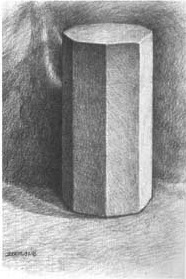
\includegraphics{Pic/SCP-001-4-1.jpg}\\
  \caption{八棱柱}\label{fig:SCP-001-4-1}
\end{figure}

大家是不是对于日记当中那些文字很奇怪呢?那其实是苏格兰古英语来着。。。

ane bouned jew'l of onycs and filigree gold, of fineneſs beyond rational ſtatement

a bitter, blaſted place, older than days

a fearſome death god

ſelections of curious providence

可以看到s全部变成了长s:ſ。还有一些几乎无人使用的词语。。。查了好久

古怪的地方:里面说SCP-001不会被任何辐射穿透,但电子显微镜的工作原理就是用辐射穿透物体再观测。。。或许是接受反射回来的辐射的信息吧,毕竟那些黄金是包裹在玛瑙上,突起来的。

宇宙微波背景辐射在03年观测到的图片:\vspace{12pt}

现在的宇宙照片大多是个横放的椭球,但这里的南北极点却是相对于一个鸡蛋样子的宇宙来说的:
\begin{figure}[H]
  \centering
  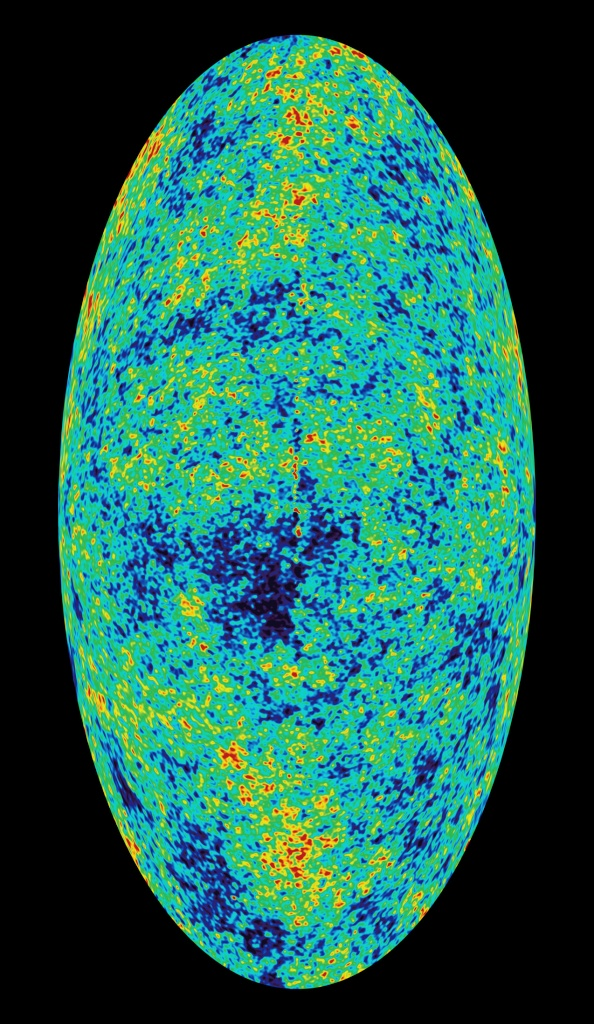
\includegraphics[width=100pt]{Pic/SCP-001-4-2.jpg}\\
  \caption{宇宙微波背景辐射}\label{fig:SCP-001-4-2}
\end{figure}

关于宇宙微波背景辐射和温暖:宇宙微波背景辐射(又称3K背景辐射)是一种充满整个宇宙的电磁辐射。频率属于微波范围。是大爆炸后残留下来的余温。在宇宙各处都可以观察到相同的辐射。也就是说,真空是有温度的,大约为-270.15摄氏度。每件物体只要有温度都会放出辐射,只不过冷的物体放出的辐射比其他物体给与它的辐射少,热的东西则相反,所以热量从热到冷流动。而SCP-001完全惰性(这在物理学上是不可能的)又会放出3K辐射,也就是说它不完全接受热量而放出热量,会比所有碰到的物体高3度。人36.5度摸上去就是39.5度,工业炉5000度它对于工业炉就有5003度。所谓温暖实际上是这样引起的。
然后是一个历史知识:苏美尔楔形文字在1400s就已发现,但当时未能破译。直到1802年才由德国教师格罗特芬德破译。再看看馆长翻译的时间:1805……

\addtocounter{mychapter}{1}
\chapter[SCP-001 工厂]{SCP-001 Dr. Bright's Proposal - The Factory \\ SCP-001 工厂 \protect\footnote{本篇翻译为繁体,编者将其简体化方便阅读} \\ 翻译:忘我竹}\label{chap:SCP-001-5}

{\Large\color{red}SCP-001:O5}\vspace{12pt}

本文是一位O5的口述记录。\vspace{12pt}

晚上好,博士。\vspace{12pt}

不,不,不用站起来。对,没错,我就是那个人。既然你我都明白,我们还是不要在这件事上耽搁太久了。你只知道我的号码,而我对你的瞭解能让我造一个你的复制品,连你妈都分不出来谁是真的。不对,这不是一个威胁,只是一个事实。\vspace{12pt}

现在,关于我为甚么来到这里,你似乎碰巧发现了一些在你的权限之上的东西。恩,不对,碰巧发现不是一个正确的词。发掘?或许更准确。而你正在接近一个危险的临界点,到那时任何进一步的发掘都会以一个致命的枪伤作为句号。这对于我们的事业将会是个可悲的情形,因为除此之外,你依然是一个非常棒的研究员。因此,你将会得到只有极少数基金会中人曾得到过的东西:一个解释。\vspace{12pt}

没错,当你第一次探索SCP-001时,我们就已经警惕了。每一个曾短暂接近它的研究员都会忍不住往里面看看。大多数都满足於他们发现了带着火焰剑的天使,它已经埋在足够深的等级下了。但接着你开始调查The Factory,我们就知道你不会停下。所以,我将告诉你那个清晰而简单的答案。\vspace{12pt}

The Factory就是SCP-001。\vspace{12pt}

但这个真相是永远不会被写下来的。这是我早在基金会创立初期就决定的,而且我仍然坚持这个决定。你们这些研究员实在太有好奇心了。我不知道哪件事更令我恐惧:我们永远不会瞭解The Factory,还是我们有一天会瞭解它。好吧,我知道你渴望知道更多。\vspace{12pt}

The Factory是在1835年建立的。那时它叫做The Anderson Factory,因一位非常富有企业家,其创始人詹姆士・安德森(James Anderson)而得名。它是,呃,我只能告诉你它是在美国成立的,并且是到那时为止最大的工厂,最宽处有一英里(1.6公里),所有建筑都有3层楼,大门前还有一个专供Anderson使用的7层高塔。\footnote{译者注:1835年的奇迹}它被设计为工厂的最终形态,能够处理所有的东西,包括员工的住房。人们可以在这里出生、工作、生活、死亡而不需要离开工厂的范围。人们的工作范围极广:从牛的养殖到屠宰,纺织,以及世界上一切工作。\vspace{12pt}

但是,没人知道James Anderson是一个撒旦的崇拜者。他有很大可能信奉一些异教的神灵。他对于工厂里建筑的位置和机器的摆放有非常严格的要求。工厂的幸存者声称建筑的地板上刻满了只有当鲜血流过时才能看到的神秘符号……当然,幸存者还告诉了我们一些其他的东西。他的钱是从工人阶级的血汗,甚至工人阶级的尸体上赚来的。他在日记里认为工人不过是一种比人类低贱的东西,放在地球上就是来为他服务的。\vspace{12pt}

当然了,在那个时候还没有人瞭解他的邪恶嗜好,因而他的工厂吸引人们蜂拥而至。有一个地方能同时解决工作和生活?好吧,人们理所应当的想要进去!至於严苛的工作时间、恶劣的工作环境,残酷成性的保安,和其他所有的一切古怪,都没有关系。工厂的工人们被迫一天工作16个小时,从日出干到日落,星期天才能停工。工人甚至没有独立的房间,要与另外8人分享房间,三班倒的轮流去睡觉,保证工厂全天有人干活。从没有人听说过医疗。如果你因为你的职责受伤了(这种事经常发生),你只会被要求继续干下去,那些伤得太重而无法工作的人会被保安拉走,没人再听说过他们。\vspace{12pt}

整整40年,安德森工厂大量制造了所有人类所需的产品。肉、衣服、武器。不会有人介意牛肉里面可能混合着人肉。別去想武器是在鲜血里淬火的。不用去管衣服的颜色是来自……呃,你懂的。确实有泄漏出去的谣言,但是那些产品那么好,干嘛抱怨呢?直到有人逃了出来。\vspace{12pt}

我从没有见过那位勇敢追求自由的灵魂,不过她想尽办法见到了格兰特总统。在1875,格兰特总统寻求我的帮助。当时我是…好吧,这不重要。我只会告诉你我是一名军人,某种军人,而且我的伙伴们也是。我们有150 位好兄弟和几位姐妹,接一些常识不会接受的工作。我们清洗过一些南部联盟的顽固份子,以及我们在南方找到的更坏的东西。于是,我们做了一些调查,并不喜欢我们看到的东西。我们闯进了工厂,承担这项重担。\vspace{12pt}

我并不完全记得那个工厂陷落的夜晚了。许多记忆在我的脑子里搅成一锅粥。一些片段常会闪现出来,有时是许多人被一根锁链拴在一起,活在死亡的边缘,你极难分出来哪块肉是谁的。孩子们活在机器的支配下,身上大部份的肉都已经被转轮、齿轮之类的机器从骨头上剔掉了。\vspace{12pt}

没事,我没事。我已经很久没有回忆这些东西了。工厂的保安并不是问题,但Anderson的作品很快出现在我们面前。他把很多受伤的工人拉走,然后,嗯,在他们身上做试验。人类,如果你还能把他们称为人的话。许多种类的手臂缝在他们身上,有些还装上了动物的身体,是超出人类最荒诞邪恶的噩梦的恐怖怪物。他们不断涌来,不能称之为活着的生物一波波的出现。那个晚上我失去了许多战友。后来我们发现了Anderson的培育地下室,一个只有8岁的小女孩被绑在墙上,被变成了-\footnote{译者注:天朝血汗工厂中枪}\vspace{12pt}

对不起。即使在超过一百年后的今天,这些记忆仍仿佛满是血色。我们找到了蜷缩在他的办公室里的Anderson,用他的肠子把他吊死在高塔的窗外。在他死亡的过程中,他不断狂笑,大叫说这不是问题,我们可以杀了他,但他的工厂,The Factory,不会停工。24小时后他仍狂笑不止,我们最终放他下来,掏出他的内脏,每件都切成四块,再把剩下的部分烧成灰烬。整个过程他一直在狂喷亵渎之词,我不想回忆那些话。\vspace{12pt}

我们用了一个星期去清理这片区域、释放工人、纪录每一件我们在地下室和昏暗的房间中找到的东西。我们拿出那些看上去有用的东西,存放在大门旁的一座房子里。尝试去弄懂每一件东西。我们有150位伙伴在那个晚上进到地狱里,只有93人出来。而一星期后只剩下71人了。\vspace{12pt}

而那些我们在里头找到的东西,我的天哪。好吧,你已经在基金会工作过一段时间了,他们应该不会让你太过惊讶。不过当时我们可是第一次看见会发射真子弹的玩具枪;能把碰到它的皮肤剥下来的摇摇;只对人体起作用的大锤;一种跑得比当时所有东西都快的骨骇马;如同暗夜亲自编织的斗篷,能让穿上它的人来到一个虚无的维度,那里有……我又失态了。我们找到了很多器具,既不可思议,也很可怖。接着我们面临著一个抉择。\vspace{12pt}

我把队伍里最高级的几个人召集来,恩,我想想,我们最好称他们为长官。我们设法去弄清楚我们接下来该干甚么。每个人都有不同的想法。Chaplain(牧师)变得有点疯疯癫癫的,觉得这些对象都是神赐予我们的奇蹟,要像对待圣物一样崇拜它们。Marshall(马歇尔)还有他的跟屁虫Dawkin(道金)认为这些是工厂造出的好宝贝,要继续制造它们然后卖给出价最高的人。Injun(印第安人),我们都叫他Bass(男低音),因为他的声音像男低音一样,说这是令人厌恶的东西,声称无论如何他都会搜寻并销毁所有他找到的东西。Smith想到我们应该先释放所有劳工然后把他们带回总统那里。我们在那里争吵了几小时,几天,想办法解决这些。至於我,我觉得我们正坐在一座金矿上面,行了別那样看着我。虽然很危险,但我们可以利用这些东西,这些对象,去搜捕那些我们曾在南方偶然遇到的骇人之物,以及其他需要全世界共同应对的怪物。让这个工厂用在正道上,一个可以收容这些东西的地方,想办法让它们为人类同胞服务,至少保护人类免受其害。\vspace{12pt}

译者注:

\begin{colorboxed}
此处几个超自然相关组织都露出雏形。

Chaplain:破碎之神教会(The Church of the Broken God)。

Marshall:Marshall,Carter和Dark有限公司(Marshall, Carter, and Dark Ltd.)。

Injun或称Bass:全球超自然联盟(The Global Occult Coalition-GOC)

\hyperref[chap:各大组织介绍]{各大组织介绍}
\end{colorboxed}\vspace{12pt}

我想你应该已经猜到接下来发生甚么了。Chaplain在一天晚上带着他的崇拜者偷偷离开了,还拿走了几件小物品。我们把Marshall撵走因为我们发现他在……滥用职权。他保证他一定会报复我们。卑贱的Dawkin该死的带领他们那群人和一些重要物品离开了。Bass和他的人努力的去点燃工厂想把这些该死的东西烧掉却徒劳无功,后来他们也走了。Smith也跑去向总统汇报。我最终让他保证会告诉格兰特工厂已经彻底毁掉了。我有一个大计划。\vspace{12pt}

当然了,想要实现一个大计划是有点困难,特別是只有12个人和你一起工作的时候。不过我们还是开始了。\vspace{12pt}

计划运行得很顺利,暂时的。我们已经有了这些神奇的玩具,想要招人跟我们一起工作就变得很容易了。在那个时候,离开电就像走出村子一样简单。我们知道我们需要甚么,也知道我们会变成甚么。\vspace{12pt}

Leventhal(利文萨尔)开始得到我们的支持。他搞了个小发明,弄到了一大笔投资,都很有用。White(怀特)和Jones(琼斯)则开始得到我们⋯⋯其他人的支持。在我们搞定工厂之前的工作中我们已经发现了一些与某些人有关的有趣的东西。那些当权者不会想要泄漏出去的秘密。而且,因为我们新的根据地让我们能更好的守住这些秘密,越来越多的人跑来想让我们处理他们的秘密。勒索是个肮脏的词,不过很管用。Bright (布赖特),Argent(阿金特\footnote{译者注:意思是银})和Lumineux(陆敏讷\footnote{译者注:法语意为光辉的})著手纪录项目。Light(赖特)和Bright(布赖特)的老婆,她们是护士,确保我们保持健康。嘿。算了,只要记住Light 就可以了。在那个时代,她在卫生方面有著许多独特的见解。Czov (克佐夫),Fleischer(弗雷歇尔\footnote{译者注:德语意为屠夫})和Carnoff(卡诺夫)处理军队训练的事。Tesla (特斯拉)和Tamlin (谭琳\footnote{译者注:苏格兰妖精英雄的名字})负责找出利用项目的方法,在不会暴露我们的情况下。\vspace{12pt}

我们的效率高得惊人。一个城市围绕着the Factory建立起来了,我们开始叫它作Site Alpha,而且它还是自给自足的。特工、研究员、各种熟练技工……当然,我们不依靠那些当权者,而是靠这些工作人员。我们不断发展壮大。\vspace{12pt}

……\vspace{12pt}

不好意思,我已经是一个老头了。我知道我不愿意正视它,不过我的身体在撒谎。我的脑袋……并不总是记得准确。有时我会沈浸在回忆里。事情变得令人困惑。不过在很长一段时间里,一个显而易见的事实是:我们在利用the Factory。总是能在里面找到更多的空房间去储存东西。那个时候我们还用“东西”来称呼它们。不需要跳过这段,不需要。我们认为我们已经驯服了the Factory。这是我不停止这项工作的原因之一。但如果现在有甚么事情是我确信的,那仍然是人类永远不能驯服这些东西。收容它们就好了,就像那位你我都曾见过的Able一样,驯服它们?不可能。\vspace{12pt}

大约十年之后,我们已经组织的很好了。13位创始人只用编号作为代称,不再用名字。大家都知道怎么样让事情运转良好。并且,如果有一两件东西在the Factory里消失了,依然如此?而且有时是D级人员消失?甚么?没错,我们那时就已经有D级人员。递过来就用掉了\footnote{译者注:Disposables:一次性用品,尤指纸尿布。意译一下}。这就是字母D的由来。肯定要有一些人给我们试验那些东西,Tesla和Tamlin 对此非常坚决。但是,没错,有时我们会失去一些无关紧要的人。Adam……抱歉,是Dr. Bright喜欢说这是the Factory在让我们“留下买路财”。你不可能甚么都不付出就有收获。\vspace{12pt}

到了1911,一切都失败了。那些家伙……我们称之为小仙子。那些家伙全族都栖息在我们旁边。它们看上去跟你我长得一模一样。唯一明显的区別在于对铁过敏。对,这就是为甚么我们叫它们作小仙子。不过,你从没听说过它们是很正常的。为甚么?因为那个时候基金会就已经把它们全族都灭绝了。连根带叶的。并且我也动手了。\vspace{12pt}

我们已经被它们当成猎物一段时间了。我们之前也碰到过它们几次,都把它们成功搞定了。所以,当某位王室成员来向我们寻求帮助时,我们当然会想要让他们欠我们人情。人人都喜欢让別人欠自己人情的。我们派了一对人员去帮忙,稍微关注了一下,觉得这不过是一次狩猎派对。下次我们看见队员们和那个王室成员,他们的头都被插在杆子顶,系在小仙子骑的生物的马鞍上,它们来攻击the Factory了。\vspace{12pt}

很可怕。\vspace{12pt}

三个字,信息量太大了。我从来没有……抱歉,请给我一点时间。我从来没有告诉任何人这个部分。你应该觉得你很幸运。而且,如果你把我将要告知你的事情的任何一点点说给其他人,我不仅仅会杀了你,还会干掉那些跟你分享DNA的人,用我能想到的最可怕的方式。跟我那时会在你身上干的事情比起来,你会觉得110蒙托克程序(Procedure 110 Montauk)不过是在花园里散散步而已\footnote{译者注:咦,难道不是在花园里散步吗?相关条目:\hyperref[chap:SCP-231]{SCP-231} Special Personnel Requirements}\vspace{12pt}

我们输了。那些家伙冲了进来,毁灭了我们。骑在我们的炮台上,屠杀我们的人员,无视我们的武器就像它们不存在一样。我眼睁睁看着我左右的13位伙伴倒下,只是努力的想要保护the Factory。那我呢?我,他们的领导者,他们的朋友,他们的父亲般的长者?Bright四个孩子的教父,知己,有时是情人\footnote{译者注:个人推测O5-1给Bright戴了绿帽},平常是聆听他们忏悔的神父?我跑了,跑得就像一个惊恐的小男生,深入the Factory 那黑暗的五脏六腑中。我被那些家伙追着,只有一步之遥。我甚至能听到他们跟在我后面,感觉到他们脖子上的气息,然后……\vspace{12pt}

我来到一扇我从没有看过的门前。黄铜大门,覆盖著一些类似阿拉伯字母的符号。我向来对语言一窍不通,特別是那些狗屎穆斯林用的鬼画符。不过我当时也管不了那么多了。它们正向我冲来,我立刻拉开门钻了进去。里面的一切……都不一样。那是一种平静安宁的感觉,似乎没有东西能在那里伤害我。光线是像这样的暗红色,不过仍然觉得正常。我耳朵里充满了稳定而持续的巨大心跳声。在我的面前,是Anderson的遗骸。接着它开口向我说话,不过我打死也不会说出确切的话。更重要的是它说的话的价值,而不是细枝末节。它给了我一个希望。他告诉我……他告诉我说每一件我们使用的the Factory出品,不论我们是用它们来做甚么,都在喂养它。帮助它成长。但是,如果那群小仙子攻陷了the Factory,它们会毁掉它,我们都不能让这件事发生。它提出一个……方案。它能清除这件事。让它从没有发生过。我们只需要献出……我们自己。\vspace{12pt}

我并不想接受。我知道这绝对不安好心。但接着,我眼前浮现他们,我的家人,我的朋友,都死了。死在那些混蛋的手上……我同意了。它笑了。然后我发觉自己又回到了城墙上,看着一大群小仙子爬过山峰。我的基金会满血复活了。我手上拿着一把武器。我就不用细节吊你的胃口了,总之我们轻松战胜了它们。接着,手里拿着那些新武器,继续屠杀它们,每处它们栖息的地方,每处它们繁殖的地方。我的O5的同志们提出了疑虑,觉得我们应该留下来一点,以免以后我们可能会用到它们……我否决了。\vspace{12pt}

我们离开了the Factory。紧闭大门。把我们的东西移出来。我们把它们的名字从东西变成了特別收容协定(Special Containment Protocols),专注於收容它们,而不是……干点別的甚么。其他人都很好奇,不过都瞭解我一定有我自己的理由。我用木板把the Factory围住。关上锁好。把它埋在成吨的碎石瓦砾下,声称它实在是太危险了。我觉得……觉得我已经侥幸逃离它了。直到我在我桌上发现了一件东西。众多能发射真子弹的玩具枪的其中一把。而且上面有著the Factory的标志。\vspace{12pt}

……我偶尔派人进去过,去查看里面可能在做些甚么。最近一次派人时,那里是空的。但我们依然继续在外面发现Factory的物品。我忍不住想到底还有多少我们没有发现。和那些使用它们,并把它们藏起来的人。我回想起那具尸体说过每一次使用物品都会给the Factory提供能量。我从没有问过他它“是给甚么的能量?”我不认为我会想要知道。\vspace{12pt}

我们献给送给了它甚么?D级人员,大部份的。你以为那些尸体去哪了?总得有个地方。尸体被我拿走,然后就消失了。所有人都觉得我是个天才,能想到解决这问题的办法。有时……有时我还不得不喂给他一些其他东西。研究员。特工。他们从不知道它正在靠近。它只是伸出手来然后把他们拉进去。\vspace{12pt}

不过,我们终究是在这里做着正确事情。不论the Factory想干甚么,不论它是甚么……我们做得对。我不得不相信这一点。\vspace{12pt}

现在你知道了。你高兴吗?我看不像。为甚么要告诉你?我正在老去,Everett。如果我死了,总要有人去继续喂它。或许你会不一样。或许你能找到反抗它的办法。\vspace{12pt}

……但我很怀疑。\vspace{12pt}

\hrule\vspace{12pt}

这篇并没有提到SCP的来源,更像是一个基金会建立史:为利用和对抗The Factory而建立。后来收容的东西越来越多……而且有被The Factory利用的可能。\vspace{12pt}

那位Brght应该只是与某位O5的名字恰好相同?或者说Bright太喜欢玩了所以被降级? 爱德华 在基金会不允许Bright博士做的事情而且他因为\hyperref[chap:SCP-963]{SCP-963} Immortality现在已经是不死之身,能从19 世纪活到现在并继续为基金会工作也不是不可能的…\vspace{12pt}

本文主要是与The Factory有联系。\href{http://www.google.com/search?hl=zh&as_q=&as_oq=factory&as_sitesearch=scpfoundation.123ubb.com}{本站所有与The Factory有关文章} 体现工厂恶劣性质的文章:\hyperref[SCP-1004]{SCP-1004} Factory Porn A片全集 \vspace{12pt}

查资料甚么的就用了半小时……

\addtocounter{mychapter}{1}
\chapter[SCP-001 螺旋路]{SCP-001 Dr.Mann's Proposal - The Spiral Path \\ SCP-001 螺旋路 \\ 翻译者:Darkequation}\label{chap:SCP-001-6}

\textbf{项目编号:}SCP-001\vspace{12pt}

\textbf{项目等级:}Embla\vspace{12pt}

\textbf{特殊收容程序:}SCP-001于[已编辑]州,Site 0就地收容。一道围篱沿著SCP-001的可观察半径筑起。为了安全起见,Site 0随时都需布署五名或以上的武装守卫以防止未经授权的进入。邻近的物理实验室也需随时运作以研究任何异常。\vspace{12pt}

一块刻有提醒标语的金属告示牌应随时维护以保持在最佳状态。任何损伤都需立即回报以进行修补。\vspace{12pt}

\textbf{描述:}SCP-001是一条位于林中的环状砾石小径。以逆时针方向行走时,路途会是持续的上坡,就算通过起始点亦然;以顺时针方向行走时,路途的上、下坡数量是相同的,而没有异常。\vspace{12pt}

存取SCP-001的实验记录需五级授权。\vspace{12pt}

监督者议会(Overseer Council)的新成员需阅读文档001-O5。\vspace{12pt}

\begin{figure}[H]
  \centering
  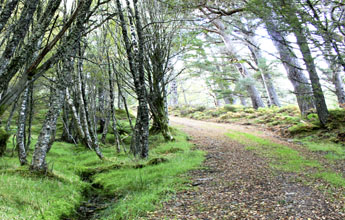
\includegraphics{Pic/SCP-001-6.jpg}\\
  \caption{SCP-001的一部分}\label{fig:SCP-001-6}
\end{figure}


\makesavenoteenv{colorboxed}% 保证盒子里的脚注正确显示
\begin{colorboxed}

\vspace{12pt}

{\Large\color{red}文档001-O5}\footnote{文本框内的脚注无法用链接形式跳转,下文如果有相同情况恕不说明。如果您知道如何能修补这个缺陷,请联系我,谢谢。}\vspace{12pt}

\hrule\vspace{12pt}

如果你正在阅读这行字的话,那恭喜你。我们的其中一员离世了。某种东西杀死了我们的一份子。或许是只怪物,或是来自GOC\footnote{译者注:全球超自然联盟,见\hyperref[chap: 同行组织]{同行组织}。}的对手。或是我们玩火自焚,像Aaron 那样。当然,不会是因为年龄。我们在那方面保持的很好,是不?无论如何,一位看守逝去了。或许是Jason,或许是Agnes,或许是我。老天,我如果不是下一个死的,我会很惊讶。我永远都是那个最操劳的。\vspace{12pt}

我写这些东西的时候,是把你当成一个人类来看待,这会是你此生最后一次受到礼遇,所以我希望你会感激。\vspace{12pt}

无论你是谁,无论你以前做过什么,你被拉进这里之前一定达到了很高的层级。你一定会发现事情有些蹊跷,不是那么单纯。我不知道你已经听过了多少,或你自己拼凑出多少。整件事的关键在于:SCP的回收与取得若不是演出来的,就是凭空捏造的。整个基金会历史上根本没有「回收」过任何的SCP。\vspace{12pt}

我应该从头开始。让我来说个故事。\vspace{12pt}

Aaron Siegel 是一名1891年在康乃尔大学进行研究的物理学家。他天赋异秉,如果没有踏上这条路的话,我想他的名字会与爱迪生、爱因斯坦跟霍金齐名。我与他非常熟稔。他曾经是,以后大概也会是,我的兄长。同时,他也是一位热忱的业馀博物学家,喜欢在森林中健行。有一天,当他正要拜访我们位于Ess.ex乡间的老家时,他遇到一条砾石小径。他决定沿著小径走一段路,并且注意到这条路不断往上延伸,远超过它应有的长度。他本该能走到附近的山丘上。但他发现自己回到原本走入的地方,而没有往下的路程。如果是另一个人,就会假设是自己感官出了问题然后离去。但,Aaron是一个顽固的人。他深入调查。他发现这条小径不遵守欧几里德的纯粹几何学。就像他之前的Saccheri\footnote{译者注:Giovanni Girolamo Saccheri(1667-1733),義大利耶稣会修士、经院哲学家与数学家,是非欧几何的先驱者之一。}一样,他找到了某种与直线性质相违的异数。\vspace{12pt}

于是他研究起这条路径。所衍生出的方程式构成了你所拿到的资料的其中一部分。你总有一天会真正理解这些文字的意义。他在附近盖了一间小屋作为临时的实验室。他的第一次实验制造了一把可以打开所有门锁的钥匙,现在被以\hyperref[chap:SCP-005]{SCP-005}的名字收容着。\vspace{12pt}

他找了其他人加入。我身为他的兄弟,自然是他首先联系的人。我那时在哈佛学医。刚开始我以为他疯了,但当他向我展示小径及钥匙的时候,我知道我必须从这里面学到更多。与我们共事的还有几个朋友与同事。他们大多都已经逝去......但,我们是一切的核心,基金会围绕著我们而建立起来。\vspace{12pt}

刚开始,我们专注于新的发现,专注于我们能做到的事情。我们有著很高的期待与抱负。我们觉得自己能改变世界、拯救众生。我们希望能喂养、庇护、医治所有的人。Thomas Carter\footnote{译者注:疑为Thomas Henry Carter(1854-1911),美国参议员。}资助我们,我们之中没有一个是穷人,但是还是钱马上就用光了。Thomas利用他跟华尔街及华盛顿的关系帮我们筹措经费。他向金主们展示了我们的一点成果,并对天发誓只会用在正途上;我兄长的未婚妻Agnes Peterson是一位懂得如何建立组织的人。我们其他人根本不晓得怎么经营一个像样的团体。是她整饬了这些梦想家与狂人,把一盘散沙、只会东奔西跑的我们组合成一个团体。\vspace{12pt}

很快地,我们建立起第一个机构。但仍然保持神秘。当我们想大声宣告自己的发现时,我们也同时害怕它们会被夺走。我们告诉自己,这都只是暂时的,等我们打好基础,一定会昭告世人。我们刚开始很小心。只制造一些小而安全,甚至很有用的道具。像\hyperref[chap:SCP-006]{不老泉}、\hyperref[chap:SCP-018]{弹力球}、\hyperref[chap:SCP-011]{内战雕像}。随著我们的信心渐增,我们开始在人类身上实验。像混凝土人就是自愿的。或是肚子里有个行星的男人,原本只是个流浪汉,但我们让他有了特点,不是吗?\vspace{12pt}

太容易了,或许从一条小小的泥巴路能找到这么多东西看来可笑,但这些发现就只是一个接著一个,不断流泄而出。这简直就像是有什么东西在背后帮助我们一样。\vspace{12pt}

但接下来,事情开始脱序。Aaron在玩弄他的方程式时,意外衍生出丟失的数字。我在实验室里,发现自己制造了\hyperref[chap:SCP-008]{僵尸瘟疫}。但我们对自己的计划太过投入,更多的研究带来了\hyperref[chap:SCP-015]{梦魇管线}还有\hyperref[chap:SCP-087]{楼梯井}。我们才知道应该找人帮忙了。Thomas对军方展示了我们的成果。告诉他们这些东西是我们「找到」、「发现」的。我们胡诌了几个名字像「普罗米修斯实验室\footnote{译者注:见\hyperref[chap:同行组织]{同行组织}}」和「混沌分裂者\footnote{译者注:见\hyperref[chap:同行组织]{同行组织}}」。 他们就以个人名义掏出大把钞票。我们茁壮起来,并且向外扩张。我们在其他国家重复这样的生意。有些人买帐,有些人不,这样已经足够了。我们成为一个国际性的组织,招募更多的研究者,但很少有人怀疑自己的实验对象是来自我们的手中。有时候我们会安排某个项目被外勤人员「找到」,有时我们乾脆直接写下报告。一张张的文件和一次次的收容失效。如果我们说一件事情如何如何,它就会是那样,直到永远。\vspace{12pt}

当然,问题还是不断产生。Jeremy跟Thomas偷走了我们的实验成果,来成立他们荒谬的俱乐部\footnote{译者注:指Marshall, Carter, and Dark Ltd.,见同行组织。}。我们的一个研究员发起疯来,开始崇拜机器\footnote{译者注:指破碎之神教会(The Church of the Broken God),见\hyperref[chap:同行组织]{同行组织}},并带著足以成为威胁的知识逃走了。我们至今仍在处理这些小组织造成的影响。\vspace{12pt}

我们遏制它们、掌握它们。我们欲罢不能,你懂吗?我们非但没有警觉,反而更加大胆。我把一个小男孩剖开,把他变成了一团憎恨的血肉。\vspace{12pt}

理由,总是有理由。比如\hyperref[chap:SCP-231]{231},我们创造了她与她的姊妹。我们从孤儿院找到它们,并写好了剧本。没有意外,我们明白自己在做什么。这件事曾经有个理由,但如果我能想起来的话,肯定会遭天谴。我们之中没有一个人知道我的兄长在哪,或他成了什么东西。\vspace{12pt}

我们继续前行。经过\hyperref[chap:SCP-076]{亚伯}、经过\hyperref[chap:SCP-354]{血池}、经过那\hyperref[chap:SCP-682]{该死的大蜥蜴},我们依旧前行。我们还能做什么?从这场由我们自己发动的灾难中幸存的唯一希望,就是深入了解它。骑虎难下也不足以形容我们的情况。但这不是我们真正担心的,也不应该是你所担心的,毕竟我们已经立足有数百年之久了。\vspace{12pt}

真正让我挂心的是那些不是由我们所创造的异常。不,我这是头一回说实话。这些东西都不是从外面回收的。但其中一些,却不是我们的成果。它们就是......某一天出现了。它们被收容著,它们一直都被收容著。你还不懂吗?事情不再由我们掌控,从头到尾都不是。
\end{colorboxed}\vspace{12pt}
\hrule\vspace{12pt}
//我发现越编辑,那些注释的号码越混乱,我也受到\hyperref[chap:SCP-033]{033}的影响了吗?

\addtocounter{mychapter}{1}
\chapter[SCP-001 遗物]{SCP-001 Dr. Mackenzie's Proposal -  The Legacy \\ SCP-001 遗物 \\ 翻译者:Darkequation}\label{chap:SCP-001-7}
\textbf{项目编号:}SCP-001\vspace{12pt}

\textbf{项目等级:}Euclid\vspace{12pt}

\textbf{特殊收容程序:}SCP-001的所有组件需分开收容于Site Zero中具备环境控制功能的保险柜中。Site Zero的地点为5级机密,唯有O5议会成员才能知悉。\vspace{12pt}

仅允许O5等级人员存取SCP-001本身、其转录以及相关资料,除非经由程序Zero。程序Zero必须在全体O5议会成员一致的直接命令下才能实施,且程序Zero的详细内容只有O5特准的人员才能获取。\vspace{12pt}

\textbf{描述:}SCP-001是两(2)个物件与三十三(33)份文件的总称,所有权属于[数据删除],又名「监督者( "The Administrator")」。\vspace{12pt}

SCP-001-01与SCP-001-02分别是[数据删除]\vspace{12pt}

SCP-001-03至SCP-001-35的文件混合了手写与打印的格式。这些文件,除了完全没有表现出随时间劣化或破损的情形外,在所有方面都表现正常。对纸张本身年代的化验则得出了不确定的结果。这些文件的内容详列于下,包括[数据删除]\vspace{12pt}

[数据删除]\vspace{12pt}

[数据删除]\vspace{12pt}

[数据删除]由于这些物件是基金会成立的推力,同时也构成了基金会的活动准则,因此这些资讯只能在O5议会的直接命令下提供给程序Zero的人员。\vspace{12pt}

\hrule\vspace{12pt}

{\color{red}\large\textbf{在O5议会命令下进行5级加密-仅允许阅读}}\vspace{15pt}

\textbf{附录001-01:}对SCP-001-01与SCP-001-02的分析\vspace{12pt}

SCP-001-01是由未知金属物质所构成的平滑装置,尺寸约22公分宽,30公分高,1.5公分厚。项目的重量与其尺寸极为不符,达8.2公斤。其上有一个小型数位显示器,并且有一个看似是某种钥匙孔的开口。由于没有可见的接缝或紧固件,目前为止,尝试拆解或分析这个装置的尝试都已失败告终。以X光或磁共振扫描SCP-001-01内部的结果显示出不确定的结果,表示装置的内部若不是太过致密以至于无法扫描,就是内部的拓扑结构有异常。

SCP-001-01的能力貌似只有显示两个指标。第一个表现为一种状态或进度条以及数字,目前进度约在23%。另一个指标是一串简单的数位计数器,当前数字为██,███。\vspace{12pt}

SCP-001-02是一把与SCP-001-01外壳相同材质的钥匙。目前推定这是SCP-001-01的启动钥匙。\vspace{12pt}

\textbf{附录001-02:}SCP-001文件的转录\vspace{12pt}

SCP-001-03是监督者的个人日志。SCP-001-04至SCP-001-35在回收时一併夹在SCP-001-03的书页中。\vspace{12pt}

\clearpage

SCP-001-03的片段,第一页:
\begin{colorboxed}
我一向很排斥写日记的点子。文件是一回事,但我从来就不知道写下个人思考过程有什么意义。我心中的科学家告诉我,总有一天某人会需要知道整件事情的始末。
\end{colorboxed}

\vspace{8pt}

SCP-001-03的片段,第三页:
\begin{colorboxed}
人们常说,万事起头难。我已经从联邦政府那里取得了足够的资金与人员,并且建立了一个能让我继续研究的组织。[已编辑]总统坚持要我交出那个装置以确保安全,但我也把话说的很清楚:我不会交出自己的所有物。
\end{colorboxed}

\vspace{8pt}

SCP-001-03的片段,第七页:
\begin{colorboxed}
不幸地,进度在这几十年间严重落后。我坚持在解答出来前不能重建科技,因为我相信除非我们能一石二鸟,否则只会加速事情的发生。
\end{colorboxed}

\vspace{8pt}

SCP-001-03的片段,第九页:
\begin{colorboxed}
我必须杀掉他们。他们瞒著我偷偷在重建那些科技。我必须在24小时内动身,这处设施从现在起就算毁了。
\end{colorboxed}

\vspace{8pt}

SCP-001-03的片段,第十五页:
\begin{colorboxed}
我不会再犯同样的错误。一想到我为了达成目的而不得不说谎,就令我感到痛心,但我不能再一次承担让他们知道真相的代价了。
\end{colorboxed}

\vspace{8pt}

SCP-001-05貌似是以喷墨印表机印刷的文件,被夹在SCP-001-03的15与16页之间。纸张本身与其他SCP-001的文件以同样的未知方式保存。
\begin{colorboxed}
来自监督者办公室的备忘\vspace{12pt}

人类的存在已经延续了数十万年,但直到最近的数千年才真正是我们的时代。我们在信史之前的无数时间中都在做什么?我们瑟缩在洞窟中,用篝火抵御黑夜,畏惧著我们所不了解的事物。不仅是因为我们不了解太阳为何升起,还有巨大而长有人头的鱼、动如活物的石头,以及仅仅看见就令人发疯的怪物。所以我们称其为「天使」或「恶魔」,在它们的盛怒下乞求饶恕并祈祷救赎。\vspace{12pt}

物换星移,它们陨落而人类崛起。整个世界渐渐产生条理。但那些无法解释的事物从未真正走出人们的视野,就像宇宙「需要」人类所不了解的事物存在一般。\vspace{12pt}

我们不会再退回黑暗、蒙昧、恐怖的夜晚。我们不会被未知所驾驭。我们会走出自己的路。\vspace{12pt}

就算其他人不知情,我们也要对抗黑暗、关住它、不让社会大众看见,这样他们才能继续活在「普通世界」的美好幻觉里。
\end{colorboxed}

\vspace{8pt}

SCP-001-03的片段,第二二页:
\begin{colorboxed}
他们的脸不断出现在我的梦境中,成千上万。那些人盲目迈向死亡,为了我。
\end{colorboxed}

\vspace{8pt}

SCP-001-03的片段,第二八页:
\begin{colorboxed}
做错了。告诉某人真相,在我离开的前一晚。得用上我带出来的剩馀医疗资源。某方面来说,我希望他瞄准我的脑袋。
\end{colorboxed}

\vspace{8pt}

SCP-001-03的片段,第四一页:
\begin{colorboxed}
这个方程式的解能构成其他解答的架构。我亲手杀死了他们。他们能想到这是出于慈悲而下的手吗?
\end{colorboxed}

\vspace{8pt}

SCP-001-03的片段,第六四页\footnote{译者在六和四中间加了一条反斜杠,疑为手误,编者擅自将其删除。如有不妥请告知}:
\begin{colorboxed}
突然想起,临走以前他们对我说的话,他们说我可能不会看到任何东西,就像睡了一觉一样。他们说谎。我亲眼看著他们被疯狂吞噬,现实的界线崩溃粉碎,然后被替换,就像它原本如此一样。我看的到所有事情。
\end{colorboxed}

\vspace{8pt}

SCP-001-03的最后片段,第六八页:
\begin{colorboxed}
终于完成了。方程式已经完备,数字也齐全了,但再一次,这个结果来得太晚了。这个小组没有时间建构解答,而我必须再一次放弃基金会。但这次我有足够的知识,确保不会再有人遭受同样的命运。
\end{colorboxed}

\vspace{8pt}

SCP-001-34是一份破损的手写文件,夹在SCP-001-03的封面与首页之间。
\begin{colorboxed}
敬启者:

首先,我为我所做的一切道歉。单单我存在于你们的世界这件事,可能就毁灭了你和你所知悉的一切。如果你现在拥有,而且正读著这份文件,那我很可能已经死了。即便如此,我也会顺手毁了这份证据,而这表示我也失败了。也就是说,我的责任现在全都落到你肩上了,而你的命运与你世界的命运现在都操之在你。\vspace{12pt}

我并非诞生在你们的世界,我是来自另一个现实,行走于平行宇宙之间的旅行者。我从哪个年代来并不重要;如果我曾经学到了任何事情,那众多宇宙所消逝的时间就会显得毫无意义。重要的是,在我原本的宇宙中,人类的文明发展到了一个极致。我们汲取星辰的能源,学到如何操纵现实本身的架构。我们能按照自己的需要摺叠时空,甚至以医学和科技征服了死亡。我们以为自己掌握了命运。\vspace{12pt}

当我们了解到凡事都有代价时,一切都已经太迟了,我们不仅会失去我们所珍视的一切,甚至殃及其他的人。操弄宇宙结构的结果,使现实撕裂扭曲,当现实的残片开始泄漏时,我们没有发现这是多重宇宙崩溃的前兆,然后反馈开始出现在我们自己的宇宙,已然无法阻止。\vspace{12pt}

我们勉强在卷入崩溃之前,启动了最后一项保险。我们集合了残存的知识,并牺牲了自己的世界将一个人送到下一个世界。这无法修补已经造成的伤害,但能为我们争取时间,找出阻止现实崩溃的方法,这个人就是我。\vspace{12pt}

如果你还没有找到,那能佐证我言论的事物很快就会开始进入你的世界。前一个毁灭宇宙的碎片如玻璃上的雨水一般滴漏进来。那些与你的理解相违悖的东西;那些没有明显意义,却被固定在时空之中的物体;那些无法被你任何手段摧毁的事物;那些能逼疯人的存在,会让你所重视的所有理论都作废。\vspace{12pt}

我所携带的,是无数世界所留下的最后遗物。在这些书页中所描述的方程式与科技带著一份阻止崩溃的希望,一份巨大代价所换来的希望。是所有牺牲与被牺牲的宇宙一路走来的,血淋淋的轨迹,只为了让剩下的人不会重蹈他们的覆辙。在这些文字被写下时,它们已经接近完成了,但时间永远与我作对。如果我无法亲眼看著这份艰苦的任务完成,那就只能靠你了。\vspace{12pt}

祝好运,

[数据删除]

监督者
\end{colorboxed}

\vspace{8pt}

SCP-001-35是一份手写的文件,被夹在SCP-001-03的末页与封底之间。SCP-001-35的字体与SCP-001的其他文件均不符。
\begin{colorboxed}
这个,就是我们的文明曾经存在过的唯一证据了。没有人真正知道当你启动保险时会发生什么事情。有些人说使用所造成的反弹会立刻撕裂我们的宇宙中剩下的部份。其他人说使用它的力量仅仅会使崩溃加速数百倍。无论哪一种方式,都只是一眨眼的事情。当你在你的目的地醒来时,我们的家园早已荡然无存。\vspace{12pt}

你已经知道这个装置只能承载一个人,而第二个小队在你离开时已经准备就绪。我只希望我们帮你争取的时间,能让你找到阻止这场灾难的方法。不然的话,这个装置也能持续记录本地现实的崩溃程度,以及装置被启动了几次,我们这么做,或许有点虐待狂倾向吧?\vspace{12pt}

当你读到这里,我可能已经死了。我很抱歉,但你一直以来就是比较坚强的那个。我没办法从容面对自己的终结。在没有你的情况下。\vspace{12pt}

我爱你。
\end{colorboxed}

\textbf{附录001-03:}SCP-001-36

SCP-001中的文件证明SCP-001-36的存在,一件电子设备或是详载著与SCP-001相关的科技和数学资料的大量文件。SCP-001-36目前下落不明。\vspace{12pt}

\hrule\vspace{12pt}

//这篇001的褒贬不一,主要争论在太过冗于的故事与薄弱的项目本身,我自己则是被35的文件萌到。

接下来一个月我会出门,所以最后一个001要等回来才能做了。

\addtocounter{mychapter}{1}
\chapter[SCP-001 数据库]{SCP-001 S. Andrew Swann - The Database \\ SCP-001 数据库 \\ 翻译者:Ground0}\label{chap:SCP-001-8}
\textbf{编号:} SCP-001\vspace{12pt}

\textbf{等级:} Keter\vspace{12pt}

\textbf{特别监管措施:}目前尚未找到一种方法可以保管SCP-001而不带有可能引起ZK级现实崩溃和其导致的可观测宇宙毁灭的风险。(参考:监管协议ZK-001-Alpha)当前的措施被限制在对关于SCP-001信息的绝对封锁上。有关SCP-001的性质或对其描述的信息都不得被提供给任何人,除了唯一的一名O5级指挥长官(目前是O5-█)以外。一切收集到的关于SCP-001的数据都须被以【已更改】的方式进行加密存储,且密钥需被分为三部分。每一名O5 级指挥人员都需记忆且只可记忆密钥的三分之一。数据只可以被在仅供O5级指挥长官阅读的非联网的视觉终端上面被解密,并且需要全体O5级指挥人员的一致同意才可进行。\vspace{12pt}

由于谍报、心灵感应、研究或者【已更改】导致的关于SCP-001的数据泄露必须被基金会不惜一切代价阻止。O5级指挥长官,作为唯一一位有权限掌控SCP-001 知识的人员,对监管措施拥有最终裁定权。\vspace{12pt}

在正常任务中接触到关于SCP-001数据的2级或以上的基金会员工可在接受询问之后被处以A级洗脑处理而不是被处决。此类事件的处理由O5级人员视情况而做出决定。\vspace{12pt}

\textbf{描述:}【数据已擦除】\vspace{20pt}

附件: 监管日志001-Alpha

日期:01/12/19██

事件:文件出现在互联网站点【已更改】。服务器已被夺取且文章作者于【已更改】被追踪到。制造了一起被伪装成煤气泄露的爆炸。没有监察到关于文件的进一步宣传。\vspace{12pt}

日期: 03/31/19██

事件:██████ ████的一份电影剧本包含可能的泄密信息和图片。剧本原作者已被【已更改】。探员成功地用一份不含有【已更改】内容的剧本替换了原剧本。电影以███ ██████的名字上映并在周末首映获得2700万的票房收入。(译注:经8楼的stwo同学考据,这部电影是黑客帝国(The Matrix),上映时间和首映票房与描述相吻合)\vspace{12pt}

日期:06/19/19██

事件: 畅销书作家█████ ████提供给了【已更改】一份描述【已更改】的小说大纲。对作者的刺杀未能成功,导致目标高调地住院治疗。O5授权允许只用A 级洗脑来阻止可能引起的进一步关注。大纲被回收并销毁。(译注:经9楼的bearpool同学考据,这位作者是著名恐怖小说家史蒂芬·金,史蒂芬·金确实在1999 年6月19日遭到过一次车祸袭击)\vspace{12pt}

D█期: o5/2█/20█z

事cde件█:基nAt金会on研█sea究e█\%20发scov

\%5B数ttt据已擦xPu██ge除\%5D\vspace{12pt}

\begin{colorboxed}
\itshape
问问你自己你是否想要知道。\vspace{12pt}

如果答案是不,那么现在你不要继续读下去了。如果你现在离开并且将这未授权的文件汇报给你的上级,表现得痛心疾首,并且声称你只读了这一小段的话,你大概能在接受A级洗脑之后留下你的小命。当然,如果你很幸运而且那些O5的老大们当时恰好不那么多疑的话。\vspace{12pt}

所以你想要知道SCP-001到底是什么?第一个能想到的答案是它是一个占位符,一个为了首要目的理论规划,和我们每天处理这些不正常玩意儿的最终原因。SCP-001 就是为什么我们必须去应付打不死的爬虫、不断膨胀的房间、多维的红色粘液池和违反物理法则的消费品。当然,考虑到这所有的一切——既致命又疯狂的玩意儿——都缺乏固有特征而又自相矛盾,大部分的研究者都确信没有办法找出它们共有的法则,更不用说找到其共同的起源了。\vspace{12pt}

他们错了。\vspace{12pt}

(上层)不鼓励(SCP间的)互动测试有很多原因,而O5们甚至是鄙视那些将不同的SCP进行牵强附会的关联的行为。O5们不想让任何一组成员同时研究稍微多一点的这些东西,这都是由于当基金会试图找出一个SCP的大一统理论时他们所发现的东西。那些研究现在大部分都已经遗失了。001-Alpha地点已经被拆除,从档案中被抹掉,员工们被洗脑和调走。除了我之外谁都没有留下,而我也不会知道这一切,如果不是因为我有着不信任基金会的服务器的习惯并且私藏了一份令O5们惊慌失措的个人档案的话。\vspace{12pt}

我是一个001-Alpha号地点的数据分析员【给O5级指挥人员的备注:别费劲找我,我完成了你们的目的,001-Alpha地点的所有原员工的身份都已经被从记录里完全的抹掉,现在你们也不会知道更多事情了】并且参与了第一次也是唯一一次试图合并基金会所有SCP数据的尝试。我的任务是负责数据的完整性。不管你们觉得这到底有多离谱,相信我,它实际上要更糟。\vspace{12pt}

忘了那些模因的SCP吧,或者是那些定义自己描述的,或者是那些只存在于信息空间里并且在数据库里造成破坏的东西吧。对基金会的网络工作的人而言,现有的这些SCP没什么特别,只不过是量多少的问题而已。真正可怕的,是数据库当中那完全不可知也无法解释的改变。\vspace{12pt}

抱歉,我错了,尽管我实在忍不住这么想。它不是当现实发生变化时数据做出的相应改变。我对于我们使用的软件的内部所知甚少,但是我知道里面有一部分遁入了我们所认为的“现实世界”当中。并且,最初所有人都认为审查追踪到的结果只是某种BUG而已。但是,明显可以看出这软件的性质,即它和那些影响叙述的SCP们之间的有意识的孤立,使得它可以去记录一些远更为重要的事情。\vspace{12pt}

那是你们、或者O5们、甚至是我们处理的大部分SCP们所看不到的,但是基金会——直至整个宇宙——处在持续的现实不稳定变化中。SCP档案令人不安的从我们的数据库中出现和消失,而档案所提到的SCP,从各方面,也和档案一同出现和消失掉。不仅仅是SCP,是人员,整个地点甚至是基金会的几十年历史都会被重写,且无法捉摸其规律。而我们自己的记忆,以及所有的研究都会确认“客观现实”和数据库里当前的情况一致。\vspace{12pt}

有一个研究员告诉我说我们好像在寻找某些拥有像\hyperref[chap:SCP-140]{SCP-140}那样的东西,只是更大一点而已。\vspace{12pt}

对的。某些非常像\hyperref[chap:SCP-140]{SCP-140}的东西,并且是无穷大的。\vspace{12pt}

我不知道谁做的分析,说不定是我做的。如果她不知道自己的发现的话可能会更快乐一些。但是她看着那些消失的和出现的事物,那些隐约的记录的改变,并且她找到了那形式和趋势,朝着黑暗、朝着有条理的叙述,朝着一个计划……\vspace{12pt}

每一个在基金会工作过一段时间的人都会知道我们生存的宇宙是一个相当混乱的地方。我们仍然相信上帝对祂的造物保持着矛盾的态度。\vspace{12pt}

但是我们最终发现确实有一个上帝,那就是SCP-001。\vspace{12pt}

而那是一群可怕的作者们。
\upshape
\end{colorboxed}\vspace{36pt}

\textbf{附件:紧急监管协议ZK-001-Alpha 仅供O5人员阅读}\vspace{20pt}

\textit{输入密钥}\vspace{20pt}

备注:

监管协议001-Alpha带有一定的导致ZK级现实崩坏事件的可能性。只可在世界末日情景或者是基金会面临毁灭的情况下被授权使用。\vspace{20pt}

在001-Gamma地点进行的研究分析和叙述了SCP-001的改变对可观测宇宙引发的影响。结论是SCP-001由多个和人类认知形式相同的个体组成,并且因此这些个体会受到模因效应的影响。由于先前的实验显示SCP数据库会引发信息反馈,我们研发了一种可能的攻击或者控制的手段。协议ZK-001-Alpha,当启动的时候,会通过软件病毒将多种模因作用剂导入SCP数据库,并且通过可观测的数据反馈,将SCP-001暴露于这些作用剂的模因效应当中。\vspace{12pt}

ZK-001-Alpha协议包含三个层面:

\begin{enumerate}
  \item 导入引发冷静和友善的模因作用剂
  \item 导入引发睡眠、昏迷或紧张的模因作用剂
  \item 导入引发死亡的模因作用剂
\end{enumerate}

鉴于SCP-001的性质和我们对它所知甚少的相互作用,目前尚无法安全的测试ZK-001-Alpha协议,并且仍然未知在没有SCP-001作用的情况下宇宙是否能继续存在。

\addtocounter{mychapter}{1}
\chapter[SCP-001 基金会]{SCP-001 Scantron's Proposal- The Foundation \\ SCP-001 基金会 \\ 翻译者:Darkequation}\label{chap:SCP-001-9}
\begin{figure}[H]
  \centering
  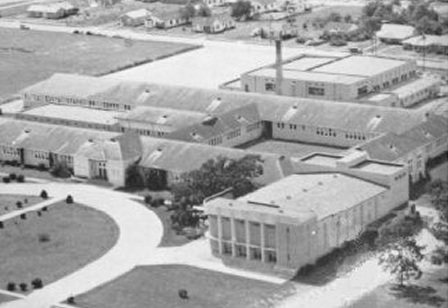
\includegraphics[width = 200pt]{Pic/SCP-001-9.jpg}\\
  \caption{CA3的空照图,摄于最初发现后两个月。}\label{fig:SCP-001-9}
\end{figure}

\textbf{UIU\footnote{译者注:Unusual Incidents Unit,联邦调查局所属特异事故处,见\hyperref[chap:同行组织]{同行组织}}档案 0041:} 位于██████, ██的变异高中校舍(Confirmed Anomaly 3,已确认异常3 号)\vspace{12pt}

\textbf{项目等级:}53(高侵入性、未知能力、未知性质)\vspace{12pt}

\textbf{特殊收容措施:}\sout{已确认异常3号(CA3)需被高于30尺的带电铁丝网所环绕,并由美国陆军第█████排守卫。任何关于CA3内部的影像资料都需尽快删除,且所有目击者都将被无限期囚禁。}\vspace{12pt}

在所有情况下都不允许人员进入CA3,或与居住其中的人员沟通。但在任何时候曾经进出CA3的人都应被囚禁与审问。\vspace{12pt}

由于控制项目的一个或多个实体所拥有的未知能力,对CA3的直接军事突击已经被证实是不可行的。\vspace{12pt}

\textbf{笔记:}这是一份摘要,不包含所有关于CA3的资讯。对CA3的详细资料请参阅UIU档案0042至0218- ██████主任\vspace{12pt}

\textbf{已知资讯:}特异事故处在1954年九月五日警觉到CA3的存在,当██████████高中的学生报告他们的校舍内部发生了前所未有的变化。\vspace{12pt}

在发现的当下,CA3表现出数个-若非原本就存在的-异常性质:

\begin{itemize}
  \item 设施内几乎所有墙壁都被钢筋混凝土所替换,某些房间则以其他材质建造,原因不明。所有对外的窗户都从内部被掩盖。
  \item 所有课桌椅、个人财物、课本,或其他公立高中应有的物件都消失了。保险柜仍存在,但尺寸明显缩小,且是由不锈钢构成。
  \item 所有房间与设施的格局、位置与尺寸都与学校原本的蓝图不符。且房间内部经常出现看似随机的修改,被改变的房间数量仍旧不明。
  \item 发现了不少于七台的计算机,每一台都使用最先进的磁芯内存。在被分类为已确认异常之前,██████████并没有计算机。计算机内的所有资料都无法存取,且机器本身都被螺丝固定住。
  \item 礼堂被大面的钢墙阻挡而无法进入。对这个阻碍进行搬移或破坏的尝试皆以失败告终。墙壁与礼堂本身的规模与用途不明。
\end{itemize}

一支被送入CA3内部以进行完整调查的小队(CA3-O5小队)没有返回,而负责寻找前一小队的第二支队伍也是(CA3-06小队)。该设施目前被封锁,等待新的收容措施。\vspace{12pt}

\textbf{更新:}在最初发现的二十三天后,守卫回报CA3发出「白噪声\footnote{译者注:White Noise,在各频率上功率都相等的“干扰”或者“噪声”}」,越接近礼堂噪声越大。五小时后,白噪声停止,但CA3 内部能听见谈话声。\vspace{12pt}

在深入调查之后,发现建筑内部现在包含了大量人员,所有人都看似漫无目的地在设施中游荡。值得注意的是,每个个体在外观上都与CA3-06的队员一致,但CA3内部的居民数目远超过CA3-06。囚禁或互动的试图因[机密]而失败。没有发现CA3-O5小队的十二名成员。此外,CA3 的内部规划与前次调查也有明显差异。其中的运作机制尚未明了。\vspace{12pt}

\textbf{更新:}在前次调查的三个月后,礼堂再度发出了白噪声。这回立刻决定进行调查。发现大多数的CA3-2(对CA3内部居民的代称)聚集到礼堂的数扇门前。一个约六尺宽的圆洞出现在钢墙上,但礼堂内部仍无法观察。在0310,一个类似[机密]的物件从洞中出现,并被一名居民带走。该物件被放置在一间教室中(在先前没有观察到其开放)。这个过程持续了八小时,每三分钟出现一个新的物件。大部分进入了不同的房间或保险柜,但没有足够的人员来追踪所有物件。\vspace{12pt}

进一步的调查显示,大部分(或全部)产生出的物件本身都具有异常的性质。一部分的CA3-2开始看守这些物件(通称为CA3-3)或对其进行各种实验。\vspace{12pt}

\textbf{更新:}在前次调查的两天后,三名雷同的武装「守卫」出现在CA3的入口附近。由于这些守卫能无视伤害或武器等级地制服所有派往CA3的队伍,无法进一步探索建筑。\vspace{12pt}

\textbf{笔记:}在守卫出现前两天搜集到的报告指出CA3-2遵循标准UIU程序来处理礼堂中出现的物件。他们对UIU标准程序的知识与CA3-O5小队一致。\vspace{12pt}

\textbf{更新:}在UIU追踪CA6的过程中,两名与特工Dixon(CA3-06的成员)相同的人从路边的车辆中出现并强行掳走了CA6,将他拖入车中扬长而去。往后八个小时对车辆的追踪发现他们直接驶往CA3。在抵达的时候,守卫迅速开关前门让车辆通过。CA6没有再被寻获。\vspace{2pt}

\hrule\vspace{12pt}

\textbf{UIU档案0042:}CA3发出的讯息\vspace{12pt}

1965年五月15日,以下讯息以摩尔斯密码发送至标准UIU通讯频道上。敏感资料已被删改,并将每个「句子」加以编排,讯息本身并未更动。
\begin{colorboxed}
  你好!我们是O5议会而且我们(确保、收容、守护)我们的行动已经为你们所知而且很高兴能做朋友。以前能当你们的一份子很好但最好是有更充足的资源(更多的资源)我们会控制住收容。我们对于守卫与囚禁的行为,在此表示诚挚的歉意,我们需要保障人员与秘密:同时也对时间上的延宕道歉,无线电讯号被一或二个SCP所阻挡。预期在短时间内会有扩张,因为我们需要礼堂以外的空间(尚可但不佳)
\end{colorboxed}\vspace{12pt}

八小时后,收到下列讯息:
\begin{colorboxed}
  扩张了!█████████联邦大楼现正运作中,需要博士守卫D人开始招募!寻找异常而且未来可能进行国际行动,研究当然可行;但跨国活动可能需要数周。此外我们O5都知道(抱歉没有O6)虽然很难探查,但媒介礼堂不是█████!再会并祝你们好运。
\end{colorboxed}\vspace{12pt}

更进一步的资讯参阅UIU档案0███:位于█████████, ██的变异联邦大楼(已确认异常10 号)\vspace{2pt}

\hrule\vspace{12pt}

//这篇用近乎魔法的方式来描述基金会的拓展,并解释O5这个名字的由来

001终于全部翻完了,接下来没有进一步的计画,可能顺著编号补缺的吧
\addtocounter{mychapter}{1}
\chapter[SCP-001 三十六使徒]{SCP-001 Djoric/Dmatix Proposal - Thirty-Six \\ SCP-001 三十六使徒 \\ 翻译者:ashausesall}\label{chap:SCP-001-10}
\textbf{项目编号:} SCP-001\vspace{12pt}

\textbf{对象类别:}人形\vspace{12pt}

\textbf{威胁级别:} 绿型(Green)|部分情况红型(Circumstantial-Red)\vspace{12pt}

\textbf{收容等级:} Euclid\vspace{12pt}

\textbf{特殊收容措施: }SCP-001个体将被收容于标准人形收容间中。任何情形下禁止将多个SCP-001个体收容于同一站点、允许其以任何形式发生互动或是得知该群体其他成员的任何相关信息。 被分派到任何单个SCP-001个体的所有人员不得得知其他SCP-001个体的存在或它们之间的联系。

除了经由批准的测试外,SCP-001项目将不会与任何其他异常物品进行直接接触。\vspace{12pt}

修订于██/██/20██: O5 特别指令A-1130-X

由于SCP-001-05死亡事件的后果,特此禁止将SCP-001项目用于任何异常项目的无效化上。必须尽全力保证SCP-001项目的生存和无恙。对SCP-001项目的寻找和收容将被最优先考虑。一但死亡事件发生,必须以最快速度开始执行衔尾蛇协议(Ouroboros Protocol)。\vspace{12pt}

\textbf{描述: }SCP-001是一组36个人形个体的集合,分别命名为SCP-001-01至SCP-001-36。在SCP-001项目之间没有任何可见的在种族、性别、年龄或宗教信仰上的统一模式。\vspace{20pt}

每个SCP-001个体自身展现不出任何异常性质。但是,任何异常物品、实体或特性在靠近SCP-001个体时都会较其原本特性发生极大程度改变:一般而言,这会导致其异常特性的削弱或是彻底无效化。那些没有被无效化的特性会被变得与具有类似特性的对象相一致。所有这些效应都是瞬间的且会在没有任何来自个体的接触下发生。这些效应的范围会在多个SCP-001个体相互靠近时扩大,其变化的强烈程度也是如此:多个SCP-001 项目有能力在不察觉到其存在的情况下将对象的异常效应无效化。\vspace{20pt}

所有的SCP-001个体似乎都本能地了解其他SCP-001个体的相关信息,一般是这个群体的总人数和其他大约二至三人的详细信息。这种了解是模糊的,这也给锁定未被收容的个体带来了困难。\vspace{20pt}

SCP-001个体的死亡会导致多种异常实体和现象在其死亡地点显现。此类显现的严重程度将会使传统收容措施根本不能实行,并造成严重事故和一系列相关破坏。被收容的SCP-001个体宣称这是因为那些死亡个体的缺失“让那些东西穿过来了”,而且随着时间推移还会有更多更严重的的事件。此外,已收容个体还宣称任何一个死亡个体都会被一个拥有相应特性的新生儿代替,但当前尚没有这样的个体被发现。\vspace{20pt}

要了解SCP-001对物品造成的值得注意的变化的列表,参看文档001-EX。对所有无效化的完整列表可以在文档001-N找到。\vspace{12pt}

\textbf{Addendum附录-01:}

已知的SCP-001成员如下:

\begin{longtable}{cccccp{200pt}}
\hline
\multicolumn{1}{c}{编号} & \multicolumn{1}{c}{人种} & \multicolumn{1}{c}{性别} & \multicolumn{1}{c}{年龄} & \multicolumn{1}{c}{当前状态} & \multicolumn{1}{c}{备注} \\
\hline
\endhead
\hline\multicolumn{6}{r}{\small{见下页}}
\endfoot
\hline
\endlastfoot
SCP-001-01 & 犹太裔德国人 & 男 & 94 & 已收容 & 当前处在人工抑制中以防止其死亡。在其左臂上印有数字表示的身份识别。\\
SCP-001-02 & 泰米尔人 & 女 & 88 & 已收容 & 收容时正处于怀孕中。孩子平安出生,当前正处在基金会观察中。\\
SCP-001-03 & 不列颠人 & 女 & 91 & 已收容 & 个体被记录是一名于1943年死亡的英国随军护士。\\
SCP-001-04 & 中国汉族人 & 男 & 97 & 已收容 & 一名全真教道士,第一个向基金会透露与其他个体相关信息的个体。\\
SCP-001-05 & 普什图人 & 男 & 101 & 死亡 & 个体于收容期间死亡。详情参见事故报告001-05-EX。\\
SCP-001-06 & 意大利人 & 女 & 39 & 未收容 & 最早被回收于布达佩斯的一处旅馆中。八天后在SITE-90的一次收容失效中逃跑。当前位置未知。\\
SCP-001-07 & 波兰裔阿根廷人 & 女 & 52 & 未收容 & 被GOI-16 “地平线倡议”控制.\\
SCP-001-08 & 俄罗斯人 & 男 & 5 & 未收容 & 被未知个人或组织控制。没有发现其家庭成员。\\
SCP-001-09 & 土著澳大利亚人 & 女 & 31 & 未收容 & 被GOI-16“地平线倡议”控制。\\
SCP-001-010 & 非裔美国人 & 男 & 28 & 未收容 & 被GOI-16“地平线倡议”控制.\\
SCP-001-011 & 尼日利亚人 & 男 & 45 & 已收容 & SCP-001-011的家人在对其进行回收的过程中出现。他的长子不顾其反对对基金会人员进行武力抵抗,被杀。其余家庭成员已接受了A 级记忆删除\\
SCP-001-012 & 阿拉伯人 & 女 & 14 & 死亡 & 在回收过程中被GOI-03“混沌分裂者”成员杀死。详情参见事故报告001-012-RC-EX。 \\
SCP-001-013 & 韩裔美国人 & 女 & 未知 & 未收容 & 尚未成功回收。 \\
SCP-001-014 & 纳瓦霍人 & 男 & 23 & 已收容 & 在对象和SCP-1295联系后被基金会人员回收。详情参见文档001-EX。
\end{longtable}

\textbf{Addendum附录-02:} SCP-001-01到SCP-001-05最初于██/██/1944在一次由HMFSCP 对耶路撒冷地区发生的疑似奇迹和其他异常事件进行的调查中被回收。SCP-001-01到SCP-001-05被发现时由三人照看,此三人分别被归为POI-1458, POI-1459, 和POI-1460. 上述三人可能与GOI-16“地平线倡议”有联系,并有可能参与了该组织的创立。\vspace{12pt}

回收尝试因HMFSCP的内部争斗被妨碍。SCP-001-01在交火中严重受伤,但还是被成功稳定住并和其他个体一起被回收,并被保护主义者派别控制。负责保护这些个体的那些人员在交火中逃走,之后再没有被逮捕到。\vspace{12pt}

\textbf{Interview Log 采访记录001-11-02}\vspace{12pt}

下面对SCP-001-05的采访记录于██/██/19██.\vspace{20pt}


Dr. ████████: 你上次说你有一个特别的使命。你能解释一下吗?

SCP-001-05: 我在这里是为了把事情纠正到位。

Dr. ████████: 请继续。

SCP-001-05: 这世界是破损的,博士。我的兄弟姐妹和我来到这里是为了将它治愈,我们集合起来并为将要到来的做好准备。进程本已经开始推进,但很遗憾出现了一些波折。

Dr. ████████: 请解释一下。

SCP-001-05: [SCP-001-01],他本是那个负责把所有其他人集合起来的人。 但因为他现在正在生死线上挣扎,这个任务落到了我们身上,但我们只能瞥见一小部分其他人。不过这本来也足够了。

Dr. ████████: 你不为他的安危担心么?

SCP-001-05: 死亡只是将要做的事的另一部分。没什么好担心的。

Dr. ████████:真是令人赞叹的处事态度。你是怎么发现自己的使命的?

SCP-001-05: 我做了个梦。预兆,预言,幻象,随你怎么叫它吧。它在我脑海中种下了一颗种子,你可能会把这叫做一种直觉。那是在我见到 [SCP-001-01] 的后一天.

Dr. ████████: 你能描述一下那个梦吗?

SCP-001-05: 那里有个男人,穿着很华丽,看起来像个国王或者皇帝。他不停地说“裁缝在哪?我的裁缝在哪?”,同时来回踱步。每一次他问出这个问题,另一个声音就会回答到“他就要来了,他就在眼前”。但是那个他并没有到来。男人变得越来越沮丧,突然一群飞蛾扑到了他身上,开始啃食他的衣服。随着越来越多的飞蛾扑到他身上,他的长袍开始磨损、腐坏,有些飞蛾甚至开始咬他的皮肤。但是突然,门开了,来了不止一个裁缝,而是许多个,由全王国最杰出的裁缝领导。国王万分欣喜,因为他明白,他们能从这群想毁灭他的飞蛾中将他解救。他找到了我,而我跟随他。

Dr. ████████: 如果你不用这种戏剧性的措辞,这就是说当你们所有人聚在一起时,这个世界就会走向终结,对吗?

SCP-001-05: [轻笑]博士,这个世界已经终结了。这只是最后一战。这世界的时辰已经到了而且已经过了,它只会被拉扯得越来越薄,直到有一天除了飞蛾什么都不会留下。但是,还是剩有一些时间。我们终能靠自己找到彼此。

Dr. ████████: 那这会在什么时候发生?

SCP-001-05: 在那平静的日子(Quiet days),博士。平静的日子,还有和平。\vspace{36pt}

\textbf{事故报告001-05-EX}

{\tiny{仅限授权人员查看:}}
\begin{colorboxed}
  {\color{red}\uline{- 安保模因: WHAT SWORD SHALL YOU CHOOSE}}\vspace{12pt}

\textbf{日期: }██/██/19██\vspace{12pt}

\textbf{地点: }Site-128 (坐标██-██.█-██.█)\vspace{12pt}

\textbf{事件类型: }LK (局部危机)\vspace{12pt}

\textbf{描述: }事件在SCP-001-05死亡的瞬间,当地时间22:12发生。驻扎于 Site-41, Site-98, 和 Site-203 的所有MTF小组立即展开回应。对Site-128内所有物品的清除协议于22:15被批准。\vspace{12pt}

\textbf{产生异常}\vspace{12pt}

\begin{itemize}
  \item UAP-████ - 近似由粘土构成的自我复制实体,一旦接触到有机脊椎动物,实体会整个包裹住宿主,控制宿主的行为。若周围没有宿主,实体会平铺伸展或聚合成大团物质。
  \item UAP-████ - 长有八只羽翼、带有鸟类和头足类特征、展翼后长70M、高45M的实体。同时显现出大群外表类似乌鸦或渡鸦的实体,每个长约3M。
  \item UAP-████ - 一系列共109个巨型立方八面体,每个宽约1M。以每个对象为中心半径20M范围内空气温度提升到超过250度。受影响区域会在脱离影响范围后立即冷却下来。对象能以大约25KM每小时的速度飞行。
  \item 9次被记录的3级生物复活情景。
  \item 大范围的市民自发仪式性食人报告。
  \item 从最初事件站点延伸出约110KM范围内的异常天气模式。降雨中含有大量致命病原体,包括扎伊尔埃博拉病毒、大肠杆菌和重型天花。
  \item \hyperref[chap:SCP-1348]{SCP-1348}消失. 参见文档001-EX。
\end{itemize}\vspace{12pt}

\textbf{回收尝试:} 衔尾蛇协议于 22:23实施,在21:00完成。协议以97\%有效率被执行。\vspace{12pt}

\textbf{基金会伤亡:} 1350

\textbf{物品遗失: }27

\textbf{预计平民伤亡:} 10000
\end{colorboxed}

\vspace{20pt}

\textbf{Incident Report 事故报告001-012-RC-EX}

{\tiny{仅限授权人员查看:}}
\begin{colorboxed}
{\color{red}\uline{- 安保模因: THROUGH THE LONG NIGHT}}\vspace{12pt}

\textbf{日期:} ██/██/20██\vspace{12pt}

\textbf{地点: }[已编辑], 东萨莫色雷斯伊斯兰共和国(Islamic Republic of Eastern Samothrace)\vspace{12pt}

\textbf{事件类别: }LK (局部危机)\vspace{12pt}

\textbf{描述:}

对SCP-001-12的回收被定在当地时间07:31执行。对象勉强地表现出合作。在07:43,来自GOI-03"混沌分裂者"的特工对回收小组发起袭击。SCP-001-12在事件中受重伤, 还有特工████ 和████████。SCP-001-12这时开始语无伦次,表现出言语不清的症状:对对象当时的胡言乱语的记录如下:\vspace{12pt}

\textit{它们饿了,你看....又咬又叮又嘎吱嘎吱嘎吱嚼.....不新鲜的食物总比没有好,明白了吧?它们非常饥饿,而且会越来越饿。}\vspace{12pt}

回收小组在08:15受到第二次攻击,SCP-001-12死亡。\vspace{12pt}

\textbf{发生异常:}

\begin{itemize}
  \item UAP-████ - 高约50M,长200M的半无定形四足实体,能抵抗常规武器攻击。
  \item UAP-████ - [资料删除]
  \item 由大量蛆产生的自发性人体崩溃(物种未知)。
  \item {[资料删除]}
  \item {[资料删除]}
  \item 突然出现的洪水,由2\%巧克力牛奶、原油、鸡肉汤和兔粪便组成。
  \item \hyperref[chap:SCP-1348]{SCP-1348}再次出现. 值得注意的变化参见文档001-EX。
\end{itemize}\vspace{12pt}

\textbf{回收尝试:}监督者议会于08:17批准核武器调度。衔尾蛇协议于08:46实施,于07:30 完成。协议以61\%有效效率被执行。\vspace{12pt}

\textbf{附注: }考虑到因衔尾蛇协议实施过程中的瑕疵造成的现实不稳定,东萨莫色雷斯伊斯兰共和国已被归类为\hyperref[chap:SCP-1173]{SCP-1173}。\vspace{12pt}

\textbf{基金会伤亡:} 8

\textbf{预计混沌分裂者伤亡:} 25

\textbf{预计平民伤亡: }175,000
\end{colorboxed}

\vspace{12pt}

\textbf{文档001-EX}

{\tiny 仅限授权人员查看}
\begin{colorboxed}
{\color{red}\uline{- 安保模因: WE SAW THEM WALK ON CLOUDS OF MEAT}}\vspace{12pt}

\textbf{实验记录}001/361

\textbf{前言:} 由于SCP-001可能具有亚伯拉罕系根源,并可能对与其起源相近的宗教背景异常事物产生潜在的影响,需要进行一个确认其影响是否存在更广泛基础的测试。\hyperref[chhap:SCP-361]{SCP-361} 因其危险系数低、属于非亚伯拉罕系的宗教项目且其效应易被观察而被选中进行测试。

\textbf{<记录开始>}

SCP-001-02被引导以一块羊肝碰触\hyperref[chhap:SCP-361]{SCP-361}。

\textbf{SCP-361:} 欢迎来到HarusCo! 我们-噢,怎么是你。

\textbf{SCP-001-02:}看起来是这样。

\textbf{SCP-361:}好吧,如果是你在***,这就意味着.....该死。时辰到了。

\textbf{SCP-001-02:} 是的。

\textbf{SCP-361:}好吧,我们本来觉得我们应该能看着它到来的。来往最近已经变得很少了。也许是时候出发了。

\textbf{SCP-001-02:}你们将会和我们一起去往那里,就在一切再一次回归秩序时。

\textbf{SCP-361:} 就算你有能耐这么做吧。好吧,孩子,我们也许是时候说再见了。我们的老大和你的老大并不总是有一致的看法,但是总得说来我们还是一起度过了一段愉快的时光。那真的很愉快。

\textbf{SCP-001-02:}你会去到那里的,我保证。

\textbf{SCP-361:}而我们也绝对不曾怀疑你相信这一点。在另一边再见,孩子。或者,不见。

\textbf{SCP-001-02:} 呵. 我都记不得上一次有人叫我“孩子”是什么时候了.

\textbf{<谈话结束>}

\textbf{结语: }在测试001/361后, \hyperref[chhap:SCP-361]{SCP-361}停止活动。所有试图引起其原本常规反应的尝试都只收到了一种类似不连贯拨号音的声音。\vspace{12pt}

\textbf{实验记录}001/738

\textbf{前言: }\hyperref[chhap:SCP-738]{SCP-738}由于可能的关联性被选中进行测试。SCP-001-03没有给出实体(下文称为SCP-738-4)的外貌描述。

\textbf{<记录开始>}

\textbf{SCP-738-4: }好吧,看看谁来了!最近过的怎样?我能为您做点啥?

\textbf{SCP-001-03:} 传个信,Jack。下一次你回去的时候,告诉所有人做好准备。契约即将终止。

\textbf{SCP-738-4:} 你在唬我吧?这真不是某种骗傻瓜的烂把戏?

\textbf{SCP-001-03:} 绝对不是。

\textbf{SCP-738-4:} 真的是时候来点大事了,嗯?我操他个烂***居然已经这么久了!!你猜怎么着?对你,免费。这次我请客。这可完全是出于我那颗枯萎黑心的善意。

\textbf{SCP-001-03:}好吧,也许不是那么黑。

\textbf{SCP-738-4:}[狂笑,猛敲桌子]你这是要把我乐死在这里!看,这就是我喜欢你的原因:你总是带来欢笑。

\textbf{<记录结束>}

\textbf{结语:} 由SCP-738-4留下的契约上写着“本次店家请客。—X”。SCP-001-03没有对为什么称SCP-738-4为“Jack”作出解释。\hyperref[chhap:SCP-738]{SCP-738}当前再被使用时没有展现出异常效应并已被归类为SCP-738-N。\vspace{12pt}

\textbf{实验记录}001/1295

\textbf{前言: }于██/██/████, 18:03, 当所有四个\hyperref[chhap:SCP-1295]{SCP-1295}个体正要离开餐馆的时候,一个人突然叫住了它们,后来此人被编为SCP-001-014。由于对\hyperref[chhap:SCP-1295]{SCP-1295}的收容措施不允许基金会人员在场景中于\hyperref[chhap:SCP-1295]{SCP-1295}发生直接接触,作为代替对对话进行了记录。

\textbf{<开始记录>}

\textbf{SCP-001-014:} 先生们,我能占用你们一点时间么?

\textbf{SCP-1295-4: }哎哟喂,看看那谁总算是来了!小伙子,你知道我们等你现身有多久了?什么东西耽误了你这么久?

\textbf{SCP-001-014:} 我很抱歉。我只是最近才发觉我的职责所在。

\textbf{SCP-1295-1: }噢,别在意,孩子,Dwight就是有点语无伦次。他其实是想说能见到你真的是太好了。

\textbf{SCP-1295-2: }赞成。坐在这一点都不舒服,还只能吃一大堆水果酥皮饼直到腻了为止。是时候回到正事上了。

\textbf{SCP-001-014: }那正是我来此的目的。你们骑乘的时刻就要来临。我被授予任务来通知你们并让你们开始准备。我被告知你们知道该做什么。

\textbf{SCP-1295-3:} 我们当然知道,我的孩子,我们当然知道。不是我自夸,没有人比我们知道的更清楚。

\textbf{SCP-001-014:} 请允许我提醒你们我们生活在不同的时代里。这个任务需要的是外科手术刀,而不是大砍刀。此时此刻,你们需要做的温和一些。

\textbf{SCP-1295-1:}该死. 我就怕你会说这个。

\textbf{SCP-1295-4:} 别担心。我们会做的像随人差遣一样温和。我怀疑在所有这些完成以前我们会再见面的,我的孩子。你得自己小心。[对SCP-1295-1到3] 来吧,伙计们!时间不等人,我们还有一大堆事要准备!骑行吧!

\textbf{<记录结束>}

\textbf{结语:}所有四个\hyperref[chhap:SCP-1295]{SCP-1295}个体接着离开了餐馆。在他们离开后,基金会人员拦住SCP-001-014并将其逮捕,没有造成更多事件。从这次谈话后再没有\hyperref[chhap:SCP-1295]{SCP-1295}回到这家餐馆或是被人目击到。\vspace{12pt}

\textbf{实验记录}001/1348

\textbf{前言:}在SCP-001-05死亡后,Site 87的考古学收容单元(Archaeological Containment Unit)经历了一次DK级(维度改变)事件,站点凭空消失并变得不可从外部进入或通信。在SCP-001-12死亡后,Site 87回到了原来的位置。站点一回归,移至探索小队被立即派去调查\hyperref[chhap:SCP-1348]{SCP-1348}的收容状况,并发现其运转发生了如下变化:
\begin{itemize}
  \item 所有在站点消失时在场的基金会人员全部消失,一起消失的还有他们的个人设备、电子仪器和食物配给。
  \item 5个新的SCP-1348-1个体出现在\hyperref[chhap:SCP-1348]{SCP-1348}的内室中。不像之前被发现的SCP-1348-1-E,这些新个体看起来完全健康。上述个体被发现在进行SCP-1348-2仪式。
  \item 被编为SCP-1348-2的仪式发生了改变,这似乎是因为之前提到的SCP-1348-1的出现。由SCP-1348-1进行的修改版SCP-1348-2缺乏之前版本所具有的模因效应。由于SCP-1438-3的帷幕当前已经永久性打开,修改过的SCP-1348-2的用意当前尚不明确。
  \item 被编为SCP-1348-3的内室发生了值得注意的变化。室内原本完全是原始闪米特风格的装饰现在包括了来自多种文化风格的图案,包括中美洲、原始印欧和南极风格,此外这些图案明确地起源于距\hyperref[chhap:SCP-1348]{SCP-1348} 可能建造时期很长一段时间后的某些时期。
  \item SCP-1348-3中心的帷幕现已永久性打开并被发现空空如也,除了一些刻在帷幕内部的阿姆哈拉语蚀刻:“他已经受了太多太多的苦难,已经把这世界的重担扛在他破损的背脊上太久太久,现在终结到来,既是他的,也是这世界的。无论终结将是怎样,只需知道他已自由,终于在湮没的怀抱中进入梦乡。而这一切都是他应得的。”
  \item 没有发现辐射痕迹。重分级为Euclid的申请正在等待批准。
\end{itemize}\vspace{12pt}

\textbf{实验记录}001/073

\textbf{前言: }基于与\hyperref[chap:SCP-073]{SCP-073}互动的相对安全性,与SCP-001-11的互动测试已被批准以求找到无效化\hyperref[chap:SCP-076]{SCP-076}的方法。

\textbf{<记录开始>}

\textbf{SCP-073: }你好.我们以前见过吗?

\textbf{SCP-001-11:} 不,我们未曾谋面。

\textbf{SCP-073:} 你看起来不像是个博士.....

\textbf{SCP-001-11:} 就职业而言我是个学校教师,虽然这无关紧要。你已经从你的束缚中被释放了。

\textbf{SCP-073:}是这样么?已经过去了这么长的时间.....

\textbf{SCP-001-11:} 确实如此。

\textbf{SCP-073:} 那么,有个很简单的测试方法。你能不能… [\hyperref[chap:SCP-073]{SCP-073}转过头来,朝向他的脸。SCP-001-11点了点头,然后猛拍了一下\hyperref[chap:SCP-073]{SCP-073}.动作成功地触到了对方,没有反射被记录到。]

\textbf{SCP-073:} 确实是这样。你和我的兄弟谈过了么?

\textbf{SCP-001-11:} 不,还没有。

\textbf{SCP-073:}噢。那你见到他的时候,告诉他我很抱歉。

\textbf{<记录结束>}

\textbf{结语:} \hyperref[chap:SCP-073]{SCP-073}当前没有表现出任何异常性质并已被归为SCP-073-N,对其的观察仍在继续。\vspace{12pt}

\textbf{实验记录}001/076

\textbf{前言:} 基于将\hyperref[chap:SCP-073]{SCP-073}暴露给SCP-001-11的成果,O5议会批准对\hyperref[chap:SCP-076]{SCP-076}执行清除。SCP-001-11被安排在内层安全保护室等待直到SCP-076-2从SCP-076-1中出现。

\textbf{<记录开始>}

[SCP-001-11进入\hyperref[chap:SCP-076]{SCP-076}收容室,被指引等待SCP—076-2出现。63分钟后,SCP-076-2从SCP-076-1中出现。一见到SCP-001-11,SCP-076-2突然发出一阵狂笑并痛哭了近30分钟。]

\textbf{SCP-076-2: }他原谅我了么?

\textbf{SCP-001-11:} 是的。

\textbf{<记录结束>}

\textbf{结语}SCP-076-2当前没有展现出异常性质或暴力行为,已被归类为SCP-076-2-N。它已被迁至一间高等级安保人形收容间中。

\end{colorboxed}

\vspace{12pt}

\textbf{文档001-IC-34}

{tiny 仅限授权人员查看}

\begin{colorboxed}
{\color{red}\uline{- 安保模因: ON BASALT FEET WE STOOD}}

下面的公告来自GOI-16"地平线倡议"的领导层。信息在██/██/20██对物品 E-7455的回收中被发现于其侧面\vspace{12pt}

你要怎么向别人解释这世界正在死亡,而他们是唯一可能解救它的人?\vspace{12pt}

自从在耶路撒冷那命中注定的日子后,六十多年来我们常常问自己这个问题,并一直怀着不同的理念以最有效的方式在这么做着。50年前,我们曾是以利亚(Elijah),满怀怒吼和愤懑,号召我们越来越动摇的兄弟们共同支持三十六使徒的事业,靠恐惧来向我们的目标前进。30年前,我们曾是以赛亚(Isaiah), 希望激励我们越来越胆怯的兄弟们,于是我们向他们确证我们使命的正义,向他们诉说我们使命的伟大, 靠他们新寻到的信心来建起让我们的目标得以立足的大厦。10年前,我们曾是耶利米(Jeremiah),在世上最强大的力量面前哭诉,乞求他们来倾听,因为我们现在明白了完成这个使命已然超出了我们自己的能力之外
而现在?现在我们是约拿,而且已经无言可说。我们要怎么做才能让你明白什么是真正危急的事,当你唯一能看到的是因为三个老人的一番话,你组织所做过的一切就都将化为乌有? 就是对一个正直的人来说这也要求的太多了,何况我们还不能确认你是。但我们只求你听着。\vspace{12pt}

你已经见过三十六使徒能做什么了。你已经见过世界围绕着他们崩坏,但你不知道这是为什么。你们只是把他们当做你们的疾病之书中又一个记录,一个对你们努力维系着的整体—这世界—的威胁。并不是那样。那些你们努力向世界隐瞒的物品和现象并不是疾病,它们是征兆,而你们不能靠把它们掩藏起来来让世界重获健康,这只会让那潜藏着的问题被忽略掉。而关键在于,这个问题是长期的。这世界只是单纯地老了,而三十六使徒....他们或许能让这世界再一次年轻起来。\vspace{12pt}

他们有能力这么做,而你会被要求作出终极牺牲-你必须放弃你的身份。你被要求确保,而我们会要你相信未经证实的东西。你被要求收容,而我们会叫你去释放。你被要求去保护,而我们会要你放弃这脆弱的世界。这是个不可能的请求,这一点我们明白。但若有任何一丝希望我们就必须这么做。释放三十六使徒,让他们聚在一起。让他们做必须要做的事,而我们则会跟随。\vspace{12pt}

帮助三个老人让这世界再一次年轻起来。别让它死去。
\end{colorboxed}

\part[SCP-002 \textasciitilde\ 100]{SCP-002 \textasciitilde\ 100 \protect\footnote{由于本章从002开始,所以序号也从2开始,便于阅读和编辑。}}
\setcounter{mychapter}{2}
\chapter[SCP-002 起居室]{SCP-002 The living room \\ SCP-002\ 起居室 \protect\footnote{因为原标题名有双关义,中文里不好直接体现,本译名仅供参考} \\ 翻译者:Трагед}\label{chap:SCP-002}
\begin{figure}[H]
  \centering
  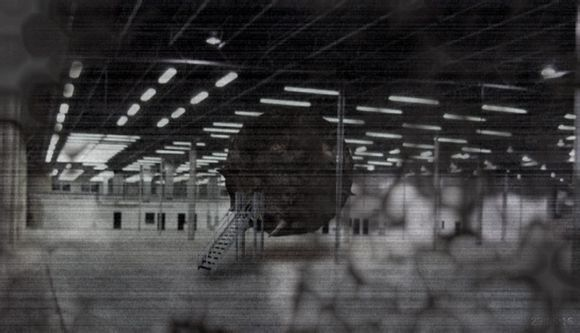
\includegraphics[width=300pt]{Pic/SCP-002.jpg}\\
  \caption{SCP-002}\label{fig:SCP-002}
\end{figure}

\textbf{项目编号:}SCP-002\vspace{12pt}

\textbf{项目等级:}Euclid\vspace{12pt}

\textbf{特别收容措施:}SCP-002必须在任何时候都能连接到电源,从而使它处在一个(处于)类似于充电的状态下。如果发生停电,立刻关闭整个设施并且疏散人员,当设备重新来电(恢复供电)时,必须要用X射线爆破和紫外线(必须交替使用X射线光束与紫外线光束)频闪这个区域,直到SCP-002重新连接上电源进入充电模式。整个封锁区须时刻保持在负气压(负压)下。\vspace{12pt}

在封锁区或者SCP-002 20米范围内(与SCP-002距离20米内)的工作队伍必须至少包含两(2)名成员。在接近SCP-002的时候(时),工作人员必须时刻保持身体接触,以确认对方和自己的感知能力是否正常(以确认对方和自己的感知是否呈现迟钝、扭曲、或由于接近目标而产生影响)。\vspace{12pt}

在封锁区或者SCP-002 20米范围内的工作队伍必须至少包含两名成员,在接近SCP-002的时候,工作人员必须时刻保持身体接触以确认对方和自己的感知能力是否正常。\vspace{12pt}

2级以下的工作人员禁止接近SCP-002,如果有两位异地的O5级别的管理员的书面授权,则可以破例进入。如果有这样的破例者,他必须全程由5位 3级安全人员保护,并且要放弃级别和安全检查,在于SCP-002接触后,指挥人员必须陪同破裂者在据SCP-002至少5公里外做一个72小时的隔离心理检测,如果正常的话,级别和安全检查将会在检测完后恢复\vspace{12pt}

\textbf{描述:}根据Mulhausen的SCP-002发现报告,SCP-002的样子类似于一个60$m^3$或者2000立方英尺的大肉球,一个铁的活动门通往其内部,内部是是一个小型的廉租公寓房间的样子, 一面墙上有一扇独窗,但是从外部却看不到,屋里放有家具,仔细观察大概是用雕刻的骨头,头发和人体部位组成,屋里的每个东西都有独立的或者断开的DNA序列。\vspace{12pt}

\textbf{参考资料:}至今为止,对象已经造成了7人消失,而且SCP-002也在研究所中体内自己产生了2个灯,一张小地毯,一台电视,一台收音机,一个气垫椅,三本未知语言的书,四个儿童玩具,一株小盆栽。用实验室动物包括一些高等的灵长类对SCP-002实验,结果都没有引起任何反应,用尸体也失败了。但是根据它的内部配置的更新,明显是在引诱活人去里面居住。\vspace{12pt}

-----------------------------\vspace{12pt}

这是关于发现SCP-002的简短报告\vspace{12pt}

此物体在北葡萄牙的一个弹坑被发现,它从轨道上撞向地球,被一厚覆盖岩层包裹着,经过冲击,它外表的肉质层被表露出来。一位当地农夫发现它后告知了村长。当此物体发出了一些小型的异常辐射后,此区域发出了4级警告,随后此物体受到了SCP的注意。\vspace{12pt}

一个由Mulhausen将军带领的SCP保安人员组成的搜集小队立刻被派遣到这个区域。在那里,他们很快地将这个物体保存在一个巨大的容器里。并对它进行了初步测试,测试人员由附近的村子招募而来。三个男人单独地进入建筑但随之消失了。发现物体这一致命属性后,Mulhausen将军发布了4A级目击者(大概1/3的村民)阻止命令以确保该物体的消息不会外泄。并且开始了对SCP设备的运输[资料被删除]\vspace{12pt}

在运输的准备过程中,四个SCP保安人员难以置信地被画在此物体的内部,画的地方也是他们瞬间消失的地方。接下来的检查发现,那个物体就像(指SCP-002)“生长”出了新的家具一样,并且内部开始变得像一个小公寓的房间一样. Mulhausen将军马上命令征用适合加入留下的SCP 保安人员的危害物质应对第三班人员。他们开始将包含SCP-002的容器放上待命中的运货船,并将SCP-002运往SCP包容设施。\vspace{12pt}

[资料被删除]\vspace{12pt}

[资料被删除]\vspace{12pt}

随着Mulhausen将军的终止命令,SCP-002现在被SCP人员监视并被带入在[机密处]的容器,在Mulhausen事件后,低于2级以下的人员会被拒绝接近放置SCP-002的容器,除非他们拥有至少两名5级人员的优先批准。
\end{document}